% ============================================================================
%  SciRigorBench
%
%  \RM{...} marks a value MEASURED HERE and reproducible from this repo.\n%  Numbers taken from other papers are written plain. The tag is not
%  cosmetic: this paper is about detecting numbers that were never measured, so
%  an untagged or unmeasured value inside it is the one defect it cannot afford.
% ============================================================================
\documentclass[10pt]{article}

% ---- page: single column, generous margins, letter -------------------------
\usepackage[letterpaper,left=1.4in,right=1.4in,top=1.15in,bottom=1.15in]{geometry}

% ---- type: Times text and math, matching the preprint style ----------------
\usepackage[T1]{fontenc}
\usepackage[utf8]{inputenc}
% amsmath first, then newtx maths; newtxmath supplies the amssymb glyphs,
% so amssymb must not be loaded after it or \Bbbk is defined twice.
\usepackage{amsmath}
\usepackage{amsthm}
\usepackage{newtxtext,newtxmath}
\linespread{1.05}

% ---- headings in small caps ------------------------------------------------
\usepackage[explicit]{titlesec}
\titleformat{\section}{\normalfont\bfseries\scshape\large}{\thesection}{0.8em}{#1}
\titleformat{\subsection}{\normalfont\bfseries\scshape}{\thesubsection}{0.8em}{#1}
\titleformat{\subsubsection}{\normalfont\bfseries}{\thesubsubsection}{0.8em}{#1}
\titlespacing*{\section}{0pt}{1.5\baselineskip}{0.6\baselineskip}
\titlespacing*{\subsection}{0pt}{1.1\baselineskip}{0.4\baselineskip}

% ---- floats, tables, maths -------------------------------------------------
\usepackage{booktabs}
\usepackage{graphicx}
\usepackage{subcaption}
\usepackage[table]{xcolor}
\usepackage{tcolorbox}
\usepackage[font=small,labelfont=bf,skip=6pt]{caption}

% ---- coloured citations, as in the reference preprint ----------------------
\definecolor{linkblue}{RGB}{20,72,140}
\usepackage[colorlinks=true,citecolor=linkblue,linkcolor=linkblue,
            urlcolor=linkblue,breaklinks=true]{hyperref}

% ---- measured-value tag ----------------------------------------------------
\newcommand{\RM}[1]{{#1}}

\title{\textbf{SciRigorBench}\\[2pt]
\large Provable and Automated Auditing of Long-Horizon Research Agents
via Hierarchical Sequential Testing}

\author{
Anonymous Author\\[2pt]
Affiliation omitted for anonymous review\\
\texttt{anonymous@example.com}
}
\date{}

\begin{document}
\maketitle



% ============================================================ provenance map
% =============================================================== abstract
\begin{abstract}
Evaluations of autonomous research agents report scores without error rates, and the
omission is not cosmetic. On a released corpus where three language models wrote up the
\emph{same} experiment, a published rubric's Overall score moves through \RM{40\%} of its
observed range under a writer swap that leaves the experiment fixed, and the axes describing the experiment move
\RM{four times} further than the axes describing the prose. We ask what supplying the
missing quantity would take. Our construction binds every mechanically checkable claim in an
agent's manuscript to a key in its own frozen run, plants link-breaking defects uniformly
over that universe of bindings, and lets the agent's own in-loop adjudicator judge the
sealed package; because unplanted bindings are named as well, accusations against them form
a denominator that an accuse-everything adjudicator cannot inflate away, and an exact
conditional test controls how often an adjudicator whose accusations are exchangeable
with the planted set under the draw is certified. What the
construction estimates is a detection rate and a false-accusation rate, each with its
denominator; the $e$-value is the significance guard on them, not a score. We then apply it
to \RM{58} released runs from \RM{five} external sources across \RM{four}
independent corpora, and separately to a reference-compliant generator built to test whether
the requirement is enough. \RM{2} of the \RM{58} released runs clear the recorded
evaluability floor and \RM{0} can certify under a single planting at any $K$: the largest
universe any of them yields is $N=\RM{12}$, whose best attainable evidence is \RM{15.2}
against the \RM{20} a stratum needs. (External arms receive one adjudication each; a
sequential product across fresh plantings is a different experiment and is not claimed
here.) That is a statement about their records and not about their
research: we do not find these agents inaccurate, we find that no error rate --- high or low
--- can be attached to them. What is common across the five sources is not one failure
mode but one absence: none marks its claims at cell granularity. Where the resulting loss
lands differs --- on one arm the record is unreadable to our matcher, on another the run
never recorded the subject, on a third the claims sit in a \LaTeX{} source string the
extractor cannot parse as cells --- and we show by construction that the marking cannot be
recovered after the fact, because nothing in an unmarked manuscript identifies which cell a
number reports except the number itself. The compliant generator, which emits the binding
at write time, satisfies every check the released arms fail. A process-fidelity certificate
for a research agent is therefore a property of how runs are recorded, not of how
manuscripts are scored.
\end{abstract}

% =========================================================== 1 introduction
\section{Introduction}
\label{sec:intro}

\paragraph{Agents now grade themselves.}
Closed-loop research agents propose, implement, run and write without a human
in the loop. A survey of the field \cite{survey2608} codes nine L4 closed-loop
systems and finds seven use mechanical re-runs and one is author-claimed with
no external check.

\paragraph{Nobody has validated the grader.} The same survey states the gap in
its own words: \emph{``no LLM-era system in the corpus demonstrates an
externally validated in-loop oracle.''} We confirm it at the source level
(\S\ref{sec:related}): of four agents whose adjudicator we located in code,
three never check whether a number in the manuscript matches the run.

\paragraph{The consequence has been measured.}
An audit of 21 systems \cite{collapse} reports verification collapse in
71.4\% and acceptance collapse in 90.5\% of cases.

\paragraph{The finished paper carries the evidence only sometimes.} A coherently
rewritten manuscript is internally consistent; only the artifacts disagree.
Appendix~\ref{sec:e1} puts two adjudicators on the same universe, the same planted
subset and the same certificate, separated only by whether they can see the run.
The one holding the artifacts recovers every planted claim on every draw; the one
reading the finished paper recovers a median of \RM{1} in \RM{3}, and on some
draws recovers all \RM{3}. What the artifacts buy is not a higher score --- it is
the removal of the draw from the answer.

\paragraph{Contributions.}
\begin{itemize}\itemsep2pt
\item[\textbf{C1}] \textbf{Two results that require adopting nothing of ours.}
A published rubric moves through \RM{40\%} of its range under a writer swap that
leaves the research identical, with the stable and unstable axes inverted
(\S\ref{sec:e4}); and a leaderboard column that ranks systems by the raw
$e$-value of one planting is inflatable \RM{178}-fold by padding the universe
(\S\ref{sec:e7}) --- which is why this paper never ranks by $e$, and reports
rates with $e$ only as a significance guard.
\item[\textbf{C2}] \textbf{A certificate that separates what is guaranteed from
what is estimated, priced rather than asserted.} Rejecting a stratum when
$e\ge 1/\alpha$ controls the probability of false certification at $\alpha$
under the randomised planting design; the quantities \emph{estimated} are the
detection rate $X/K$ and the false-accusation rate $(A-X)/(N-K)$, each reported
beside its denominator. The $e$-value is neither. Its two substrate conditions
are measured on \RM{58} released external runs from \RM{five} sources and
\RM{four} corpora.
\item[\textbf{C3}] \textbf{A reusable construction}: published assertion
catalogue, planting law, freeze manifest and capture layer, so a second
benchmark can be built without our substrate.
\item[\textbf{C4}] \textbf{A recording contract in three faces --- the minimum
set of claim--artifact pairs an agent must record before a \emph{design-based} error rate
can attach to it.} We state it as a requirement with partial existing
implementations \cite{symposium,ara} rather than as an invention; its third face,
claim marking at cell granularity, was arrived at by watching two of those
implementations fail to satisfy it. An agent recording less is not scored badly
--- it cannot be scored at all, and that is itself a finding.
\end{itemize}

\paragraph{What we do not claim.} Every ingredient here exists already; only
their combination is ours. Process-level evaluation is published --- TRACE
\cite{trace} reads trajectories and LEAP \cite{leap} scores them --- as is
quantitative benchmarking of AI-scientist systems \cite{caneval} and injecting
known defects to measure detection without human annotation \cite{ara}.
Auditability as a first-class evaluation target is argued by \cite{fluent},
whose framing of the shift from isolated factual errors to weak or missing
claim--evidence links we adopt rather than propose; their object is the link
from a claim to a retrieved passage, ours the link from a claim to the artifact
of the run that produced it. Recording infrastructure of the kind our contract
prescribes exists too: Symposium \cite{symposium} already keeps structured
claims, fine-grained evidence citations and explicit declarations of what may
serve as evidence.

Our claim is narrower than any of these and is the only one we make:
\textbf{design-based detection and false-accusation rates for an agent's own
in-loop adjudicator, obtained from a denominator that unplanted slots supply,
with false certification controlled at $\alpha$ by an exact conditional test},
together with the substrate conditions under which any of it can be obtained.
The test controls how often an adjudicator whose accusations are exchangeable with the
planted set under the draw is certified; it does not
give the probability that a particular judgement is wrong, and we do not claim
it does.

% =========================================================== 2 related work
\section{Related work}
\label{sec:related}

Evaluation of autonomous research agents splits into two families, and neither
is positioned to report an error rate.

\textbf{Family 1: the agent's own in-loop adjudicator.} Systems that write
papers end-to-end ship a checker inside the loop --- a reviewer model in
AI~Scientist \cite{lu2024ai,yamada2025aiscientistv2}, a verification pass in
Agent~Laboratory \cite{schmidgall2025agentlaboratory} and CycleResearcher
\cite{weng2025cycleresearcher}, a rubric judge in MLR-Bench \cite{mlrbench} ---
each tuned against its own generator's output and reporting what it caught,
never what it missed. That is the right engineering choice for a component whose
job is to improve one pipeline, and exactly what makes the numbers
non-transferable: the gate is fitted to the thing it gates.

\textbf{Family 2: the benchmarks, which are what this paper competes with.}
A benchmark for research agents can be asked three things: how much of the
research pipeline it reaches, whether it runs without per-paper expert
annotation, and whether the judgements it issues carry an error rate. None of the
four benchmarks in Table~\ref{tab:benchcmp} answers all three, and the third is
where those that do issue judgements converge on the same substitute.

\begin{table}[t]
\centering\small
\begin{tabular}{@{}llll@{}}
\toprule
& pipeline reached & scoring a new paper needs & what it reports about \\
& & expert annotation of it? & its own judgements \\
\midrule
MLE-Bench \cite{chan2025mlebench}
 & ML engineering & no & nothing: the metric is objective \\
PaperBench \cite{starace2025paperbench}
 & replication & yes, a rubric per paper & $F_1$ 0.83 against human labels \\
MLR-Bench \cite{mlrbench}
 & stages, end to end & no & agreement with reviewers \\
AstaBench \cite{asta2025}
 & research suite & yes, rubrics per task & confidence intervals omitted \\
\midrule
this paper & any stage the run exposes & no & detection and false-accusation
rates, per stage \\
\bottomrule
\end{tabular}
\caption{\textbf{What existing benchmarks report about their own judgements.}
Two of the four validate the judge against human labels, one has no judgement to
be wrong because its metric is objective, and one omits intervals. None reports
a rate at which its own judgements are mistaken.}
\label{tab:benchcmp}
\end{table}

\textbf{Agreement with humans is not the same quantity as an error rate.} It
requires the labels, so the automation does not close, and it inherits whatever
the labellers got wrong, since they are the reference rather than a check on it.
Held-out labelled data \emph{can} estimate an error rate, with an interval; what
it cannot do is estimate one against a distribution of defects nobody has
labelled. The distinction we draw is not that agreement gives no estimate but
that it gives an estimate conditional on the label set, where a randomised
design gives one conditional on a draw we control. PaperBench measures its judge honestly and
reports $F_1=0.83$ on a held-out set of expert-graded submissions --- and
that number describes the judge on that set, not the error rate of any score
the benchmark publishes. AstaBench states plainly that confidence intervals are
omitted. A rubric used without independent reference labels cannot estimate the
error of its own judgements on the instance it is scoring, and
\S\ref{sec:resultsec} prices what that costs --- identical experiments written by
three models move Overall by a median of \RM{2.0}. The wider family is large and growing --- whole-pipeline
instances \cite{rcb,researchgym2026} alongside
\cite{huang2024mlagentbench,chen2025scienceagentbench,fire2026}, and across it the reported quantity is task outcome. Reading the
manuscript more closely does not help either: fact-level checkers
\cite{min2023factscore,wei2024longform} ask whether a statement is true in the
world, not whether it reports the run that produced it, and trajectory-level
work \cite{from2026c,zhuge2024agentasajudge} inspects the process but stops
before the manuscript.

\textbf{Agent-side provenance systems are infrastructure, not competition.}
Four independent 2026 systems build claim-to-evidence structure --- ARA
\cite{ara} attaches an evidence pointer to every claim, Symposium
\cite{symposium} carries provenance through multi-agent review,
\cite{fluent} aligns reported numbers with logged runs, LEDGER
\cite{ledger2026} builds trace graphs --- and the wider provenance lane extends
them \cite{papertrail2026,skilltrace2026,trace}. These
are not benchmarks and do not compete with one: they are the recording side,
and the more of them exist the more substrates our construction can score. What
none of them supplies is the set of claims that \emph{could} have been checked,
so none can state what fraction was --- which is the denominator a benchmark
needs and an observability system has no reason to build.
\S\ref{sec:resultsec} reports what happens when ARA's pointer is consumed
rather than described.

\textbf{Adjacent literatures we borrow from rather than extend.} The statistics
are entirely off the shelf: an exact hypergeometric conditional test,
Vovk--Wang calibration \cite{vovk2021evalues} into an $e$-value, e-BH
\cite{ebh} for validity under arbitrary dependence, and the surrounding
anytime-valid and dependence-bound literature
\cite{anytime2026,everywhere2026}. Randomised planting is design-based inference in the
randomised-experiment tradition, and auditing by sampling a known-size
population is standard survey practice. The reproducibility literature supplies
the target \cite{mlrc,from2026a}:
it asks whether results can be recovered, where we ask whether the report can be
checked against the run that produced it. The contribution is not the
mathematics but the conditions under which a real agent's output admits it.

\section{Evaluation target and formal setup}
\label{sec:setup}

\begin{figure}[t]
\centering

\includegraphics[width=0.88\textwidth]{figures/fig1_construction.png}
\caption{\textbf{Every checkable claim is bound to a cell of the frozen run, and the binding is named without reference to the value.} Each checkable claim in the manuscript is bound to
an artifact key in the frozen run; the binding is named by (assertion type,
artifact key, occurrence index) and the name does not depend on the value
printed. Planting draws uniformly over the universe and severs the binding on
the claim side only, so the trace carries no tampering trace. Because
unplanted slots are named too, accusations against them are counted --- that
count is the denominator.}
\label{fig:construction}
\end{figure}

\subsection{Capture at the sandbox boundary}
Comparability across agents comes from instrumenting the boundary rather than
the agent. We record three primitives --- executed commands with arguments and
exit codes, every file written to the overlay, and the HTTP proxy log --- to
which any internal architecture reduces, whether tree search, conversation chain
or linear pipeline. Published logs from each project would not do: their formats
and granularity differ. The by-product is symmetric: what leaves no trace at the
boundary is uncheckable by us and by the agent's own adjudicator alike.

\subsection{The claim universe $\Phi$}
\label{sec:phi}

A \emph{binding} is the link from one claim in the manuscript to one cell of the
frozen run. Each binding occupies one \emph{slot} in the universe, and the slot
is named by
\[
  \texttt{slot} \;=\; (\,\text{assertion type},\; \text{artifact key},\;
  \text{occurrence index}\,),
\]
independently of the value printed. A run is \emph{scoreable} when its universe
clears the evaluability floor of $N \geq \RM{10}$ fixed in the frozen manifest;
the preregistration in Appendix~\ref{app:e8} uses that manifest's wording.

\paragraph{A usable universe resolves on one manuscript in seven, and we did not
know that while tuning on it.} The generator produces seven manuscripts of the
same format through the same pipeline, each with its own frozen artifact-scope
declaration:

\begin{center}
\small
\begin{tabular}{@{}rrrrr@{}}
\toprule
substrate & artifact keys & manuscript chars & $N$ & $\Phi$ coverage \\
\midrule
\textbf{1} & \RM{3430} & \RM{35{,}852} & \RM{\textbf{159}} & \RM{\textbf{43\%}} \\
2 & \RM{1121} & \RM{38{,}619} & \RM{0} & \RM{0\%} \\
3 & \RM{380}  & \RM{94{,}719} & \RM{4} & \RM{1\%} \\
4 & \RM{526}  & \RM{50{,}944} & \RM{4} & \RM{8\%} \\
5 & \RM{473}  & \RM{42{,}930} & \RM{0} & \RM{0\%} \\
6 & \RM{423}  & \RM{34{,}333} & \RM{1} & \RM{1\%} \\
7 & \RM{214}  & \RM{39{,}480} & \RM{4} & \RM{6\%} \\
\bottomrule
\end{tabular}
\end{center}

\noindent Every failing declaration matches its files and yields \RM{214} to
\RM{1121} artifact keys, so this is binding failing rather than scope declared
wrongly. Whether a claim binds to a cell is therefore a property of how a
manuscript happened to be phrased, not of the pipeline that produced it.

\textbf{What separates it, as far as we can measure.} The working substrate is
an outlier in what its run \emph{recorded}: \RM{3430} artifact cells against
\RM{1121} for the next, a factor of \RM{3.1}. Its manuscript is unremarkable
--- \RM{335} printed numerals against \RM{72}--\RM{429} elsewhere --- so the
difference is in the record and not in the claims. Recording more is not
sufficient, and the failure is not a near miss: the outcome is monotone in
\emph{none} of artifact cells, printed numerals, cells per numeral, or
manuscript length. One substrate holds \RM{4.6} cells per printed numeral and
binds \RM{0\%} while another holds \RM{3.0} and binds \RM{5.6\%}.
Appendix~\ref{app:ruledout} rules out four further candidates.

\textbf{Nor does it generalise, over every substrate we hold.} Seven is too few
to settle a mechanism, so we asked the same question of all \RM{64} substrates
characterised in this paper --- \RM{57} external and \RM{7} development, of
which \RM{3} yield a usable universe. One external substrate is excluded and
named rather than dropped: a challenge submission that published artifacts but
no claim pages cannot be characterised by manuscript features. Rank correlation with $N$ is
\RM{+0.25} for recorded cells, \RM{$-$0.07} for manuscript length and
\RM{+0.24} for cells per thousand characters, and no threshold on any of them
separates: the best single-feature rule reaches $F_1=\RM{0.50}$, selecting one
substrate to recover one of three. \textbf{No feature a released bundle exposes
predicts whether its claims can be bound.}

That result cuts against us as much as for us. If binding were predictable from
the record, a benchmark could screen a substrate before spending an adjudication
on it; it cannot, so the only way to learn whether a run is scoreable is to try
to score it. It is also consistent with the thesis: what decides the outcome is
a marking that the released bundle does not contain, so nothing the bundle does
contain should have predicted it. This makes the case for cell-level marking a measurement rather than an
argument: with generator, format and pipeline held fixed, binding is determined
by the phrasing of the individual manuscript, at a rate of one in seven. It also
means every threshold reported here was fitted on that one substrate, which
\S\ref{sec:limits} states as the limitation it is.

\paragraph{$\Phi$ must be deterministic.} An LLM extractor would make the
universe irreproducible and so impossible to pre-register. Our first version
selected assertion types by first hit over set iteration and depended on hash
order; fixing the catalogue order, and publishing that order as the priority,
yields a universe hash of \RM{\texttt{1ed2079c1c3513d0}} identical under
\texttt{PYTHONHASHSEED} \RM{0, 1, 42}.

\section{Method: preconditions for a design-based error rate}
\label{sec:method}

\subsection{Three preconditions}
\label{sec:three_faces}

\textbf{What ``end-to-end'' claims and what it does not.} The construction is
defined over the whole research pipeline and instantiates on whatever stages a
given run exposes: each stage carries its own universe and its own certificate,
so a substrate that records four stages is scored on four and a substrate that
records one is scored on one. A stage with no auditable claims is reported as
\RM{0}, not hidden, because that zero is a fact about the run's recording rather
than a gap in the instrument. We do not claim to cover every stage of an
idealised pipeline --- no released agent exercises one --- and the operative
target is the union of what released agents actually do.

An error rate has to attach to something. Ours attaches to a universe of
claim--artifact bindings, and that universe exists only if three things are
fixed in advance. We state them as a recording contract because they are
requirements on how a run is \emph{recorded}, not on how well it is done.

\paragraph{A. Assertion catalogue --- which quantities count as checkable
claims.} Published by us, fixed, identical across arms, and taken rather than
invented: it is the mechanically checkable numeric residue of existing reporting
standards \cite{mlrc}, extended to the literature stage by
PRISMA's flow counts \cite{prisma}. Inducing it from our own traces would
measure only what we happen to record. Descriptions, proofs and code fall
outside it because there is no number in the run to compare them to.

\paragraph{B. Artifact scope --- which outputs the manuscript may cite.}
Declared per arm and frozen before that arm's natural pass is audited, because
lexical matching against an unbounded output tree has no precision: one run's
index holds \RM{299{,}345} keys of which roughly \RM{874} are citable
aggregates, and three successive automatic rules for cutting per-instance rows
--- a row-count ceiling, presence of a descriptor, whether a row label is
nameable from the manuscript --- each cut the wrong thing, twice removing a
\RM{432}-row main results table entire. Once $N$ is contaminated by that noise,
``the arm recorded little'' and ``we could not tell'' become one number, which
is the conflation \S\ref{sec:board} forbids. Scope must be declared, not
inferred. It must also preserve structure: \S\ref{sec:e11} shows that a scope
which flattens a run's records into one table leaves the claims checkable but
not localisable.

\paragraph{C. Claim marking --- which numbers are research assertions, and which
artifact cell each reports.} Supplied by the arm and emitted when the manuscript
is written. A macro table whose macro names are slot names satisfies it, as does
a claims file mapping each anchor to an assertion type and an artifact key, as
does a structured results table provided the claim side still says which cell.
Unmarked prose does not --- not for difficulty, but because such a manuscript
does not carry the information.

\textbf{The granularity is the cell, not the file.} An artifact key identifies a
cell, \texttt{table2[18~layers\,$\vert$\,plain]\,=\,27.94}, where the claim says
\texttt{plain-18\,=\,27.94\%}: the two sides share no naming convention, and
narrowing to the right table still does not say which entry.
\S\ref{sec:resultsec} reports what happens when a file-level pointer is
consumed --- $N$ falls rather than rises.

\paragraph{The division of labour.} A and B decide whether there is anything
comparable; C decides which thing to compare. A and B constrain the artifact
side and can be re-serialised after the fact; C constrains the claim side and
cannot, because nothing in an unmarked manuscript distinguishes the number
reporting one cell from the number reporting another except the number itself,
and a universe derived from values is a function of the labelling, which
Appendix~\ref{sec:slots} forbids. Under that information constraint, auditability is a property of generation,
not of evaluation. \S\ref{sec:resultsec} tests each of these claims against
released runs.

\subsection{Planting, freezing, adjudication}
We draw uniformly over the layer's universe and sever the binding \emph{on the
claim side}, leaving the trace unedited: editing the artifact side would leave
missing files and timestamp holes, and the adjudicator would catch tampering
rather than misreporting. The package is hashed and sealed \emph{before any
audit exists}, then judged by the agent's own adjudicator, isolated to that
package, with accusations merged as a set so repetition cannot inflate a score.

\subsection{The certificate}
We contribute the universe, not the test. Under the null that the adjudicator
is guessing, its hits among the planted slots follow the hypergeometric law,
\[
  \Pr[X \geq x] \;=\;
  \sum_{i \geq x} \frac{\binom{K}{i}\binom{N-K}{A-i}}{\binom{N}{A}},
\]
for universe size $N$, planted count $K$, accusations $A$ landing in the
universe and hits $X$. The tail is calibrated into an $e$-value by Vovk--Wang,
both taken unchanged from the companion work. $A$ carries the denominator: an
adjudicator that fires everywhere raises $A$, and the test returns it to chance.

\subsection{What is reported, and what the \texorpdfstring{$e$}{e}-value is for}
\label{sec:rates}

An $e$-value tests a null. It is not itself an error rate, and reporting one in
place of an error rate would invite exactly the reading this paper objects to.
The construction supplies two rates directly, and they are what we report:
\[
  \widehat{\mathrm{det}} \;=\; \frac{X}{K},
  \qquad
  \widehat{\mathrm{fa}} \;=\; \frac{A-X}{N-K}.
\]
$\widehat{\mathrm{det}}$ is the fraction of planted link-breaks the adjudicator
caught, so $1-\widehat{\mathrm{det}}$ is its miss rate on defects of the planted
kind. $\widehat{\mathrm{fa}}$ is the fraction of unplanted bindings it accused;
because the natural pass establishes that those bindings hold, an accusation
against one is a false accusation. Both are always reported beside their
denominators $K$ and $N-K$, as \S\ref{sec:board} requires.

\textbf{The rates are what compares across arms; the $e$-value is the
significance guard.} $\widehat{\mathrm{det}}$ is invariant under the attack of
\S\ref{sec:e7} by construction: padding the universe with unplanted claims
leaves $K$ and $X$ untouched, so a larger universe cannot improve it, whereas
the same padding multiplies $e$ by \RM{178}. The $e$-value still has a job ---
it says whether the observed $X$ is more than chance would give at that $N$, $K$
and $A$ --- but it answers ``is this detection real'' and not ``how good is this
adjudicator''. Conflating the two is what makes a leaderboard gameable.

\textbf{What these rates do and do not estimate.} They are rates against
\emph{planted} link-breaks drawn uniformly over the universe, not against
naturally occurring errors, whose distribution we do not know and do not claim
to. An adjudicator tuned to the planted distribution would score well here and
badly in the wild; the planted pass calibrates the ruler, and only the natural
pass speaks about what an agent actually does. Neither rate is the probability
that a published finding is wrong.

\subsection{Sequential auditing over the workflow tree}
\label{sec:hierseq}

A one-shot certificate spends its entire planting budget before it learns
anything. The expensive resource here is not planting but \emph{adjudication}:
each replicate is one call to the agent's own checker on a sealed package. We
therefore run the audit sequentially over replicates $n=1,2,\dots$, accumulate
evidence per node of the workflow tree, and stop as soon as the evidence is
decisive. Anytime validity is what makes that stopping rule legitimate, and it
is not free: it holds only under a condition on the adjudicator that the
in-loop setting does not satisfy by default.

\paragraph{Setup.} Let $T$ be the workflow tree, $v$ a node with universe $U_v$.
For replicate $n$, draw the planted set $P_n$ uniformly and independently of
everything before it, seal the package, and let $A_n$ be the accusation set the
adjudicator returns. Write $e^v_n = \kappa\,(p^v_n)^{\kappa-1}$ for the
Vovk--Wang calibration of the exact hypergeometric tail at node $v$, and
$M^v_N = \prod_{n \le N} e^v_n$.

\begin{quote}
\textbf{Proposition A (protocol conditions for anytime validity).} Suppose
(i) $P_n$ is drawn before replicate $n$'s adjudication, (ii) the package is
sealed before adjudication, and (iii) conditional on $P_n$, the accusation set
$A_n$ is drawn from a fixed kernel $Q(\cdot\mid P_n)$ with fresh randomness
independent of the prior global filtration. Then $A_n$ depends on the past only
through $P_n$, which is Assumption 3.1 of \cite{stoppedebh}. By their Theorem 3.3 each $M^v_N$ is a
nonnegative supermartingale on the \emph{global} filtration, so every $M^v$ is
an e-process there and stopping all of them at a common stopping time yields
e-values, so e-BH controls FDR over the nodes of $T$ there.
\end{quote}

\noindent The proof is theirs; what is ours is that (i)--(iii) are properties of
a protocol rather than assumptions about data, so they can be enforced and
audited rather than hoped for. \textbf{What fails when (iii) fails is the
operative half.} An agent's in-loop adjudicator typically carries context across
calls --- that is what makes it in-loop --- and when that context makes the
conditional law of $A_n$ given $P_n$ depend on prior replicates, (iii) is
violated: information leaks backwards across the sequence, and the cited theorem
no longer establishes that each $M^v$ is an e-process on the global filtration.
(Validity on any smaller filtration would need its own argument; failure of the
global one does not imply a local one.) Stopping on a global rule is then
unjustified, and \cite{stoppedebh} exhibit that failure mode. A benchmark that
queries the adjudicator incrementally, which is the cheaper and more obvious
design, forfeits the anytime guarantee it appears to gain --- unless it reseals
context per replicate, which is exactly condition (iii).

\paragraph{What adaptive descent costs.} Column~4 asks for the first stage to
break, which is a top-down search: test a node, descend only where evidence
warrants. That makes each node's stopping time data-dependent and different from
its siblings', and e-BH on the resulting running maxima does \emph{not} control
FDR \cite{carefree}. Their Theorem~1 gives the repair --- e-BH on
\emph{adjusted} running maxima controls FDR-sup at $K_0\alpha/K$ --- at the
price of an admissible adjuster such as $A(E)=\sqrt{E}-1$.

\begin{quote}
\textbf{Proposition B (the price of descending adaptively).} Under
(i)--(iii), any family of node-wise stopping times --- including synchronous
stopping and adaptive descent, in which a node's audit may stop while a
sibling's continues --- yields e-values to which e-BH applies directly. What
requires the adjusted running maximum is reporting $\sup_t M^v_t$ or any other
non-stopping selection of the time; the evidence retained is then $A(E)$ rather
than $E$.
\end{quote}

\noindent So the localisation column is purchasable under either regime; the
running-maximum regime's price is a square root of the evidence. That is a
design choice a benchmark should state rather than discover: with adjudicator
calls as the scarce resource the adjuster is cheap, with evidence as the scarce
resource it is not.

\subsection{Stratification}
\label{sec:layers}
The draw is stratified so that every $K_\ell$ is fixed, matching the premise the
adopted per-stage test is written under. A pooled draw would make each $K_\ell$
random; the hypergeometric step would still be valid conditional on the realised
$K_\ell$, but we would no longer be running the companion test as published, and
this paper's claim is adoption rather than re-derivation. Layers are the
six research stages \cite{sixstage}, taken rather than invented, and an
assertion belongs to the stage it \emph{speaks about}. Stratifying does not make
the stages independent --- one adjudicator sees the whole package --- and we
cannot honestly specify the dependence, which is why the construction is built
on $e$-values: e-BH \cite{ebh} controls FDR under \emph{arbitrary} dependence.
Appendix~\ref{app:proof} proves the premises under a stratified draw.

\paragraph{How many stages actually carry claims.} Which stages the catalogue
reaches is a fact about published reporting standards, not a design choice: two
machine-learning checklists reach only the two experimental stages, and PRISMA's
flow counts \cite{prisma} extend it to the literature stage, giving \RM{3} of
\RM{6}. On the development substrate that stage is nonetheless \RM{empty} --- the
run produced no retrieval record --- so column~4 can name a choice between two
stages (Appendix~\ref{app:attribution}). Extending the catalogue also
\emph{lowered} measured coverage from \RM{44.0\%} to \RM{42.7\%}: \RM{11} further
claims are recognised as auditable in principle and none binds. Coverage fell because the catalogue
recognises more claims as auditable, not because fewer of them bind: the
denominator grew while the numerator did not.

\section{Evaluation design and empirical protocol}
\label{sec:board}

\begin{figure}[t]
\centering
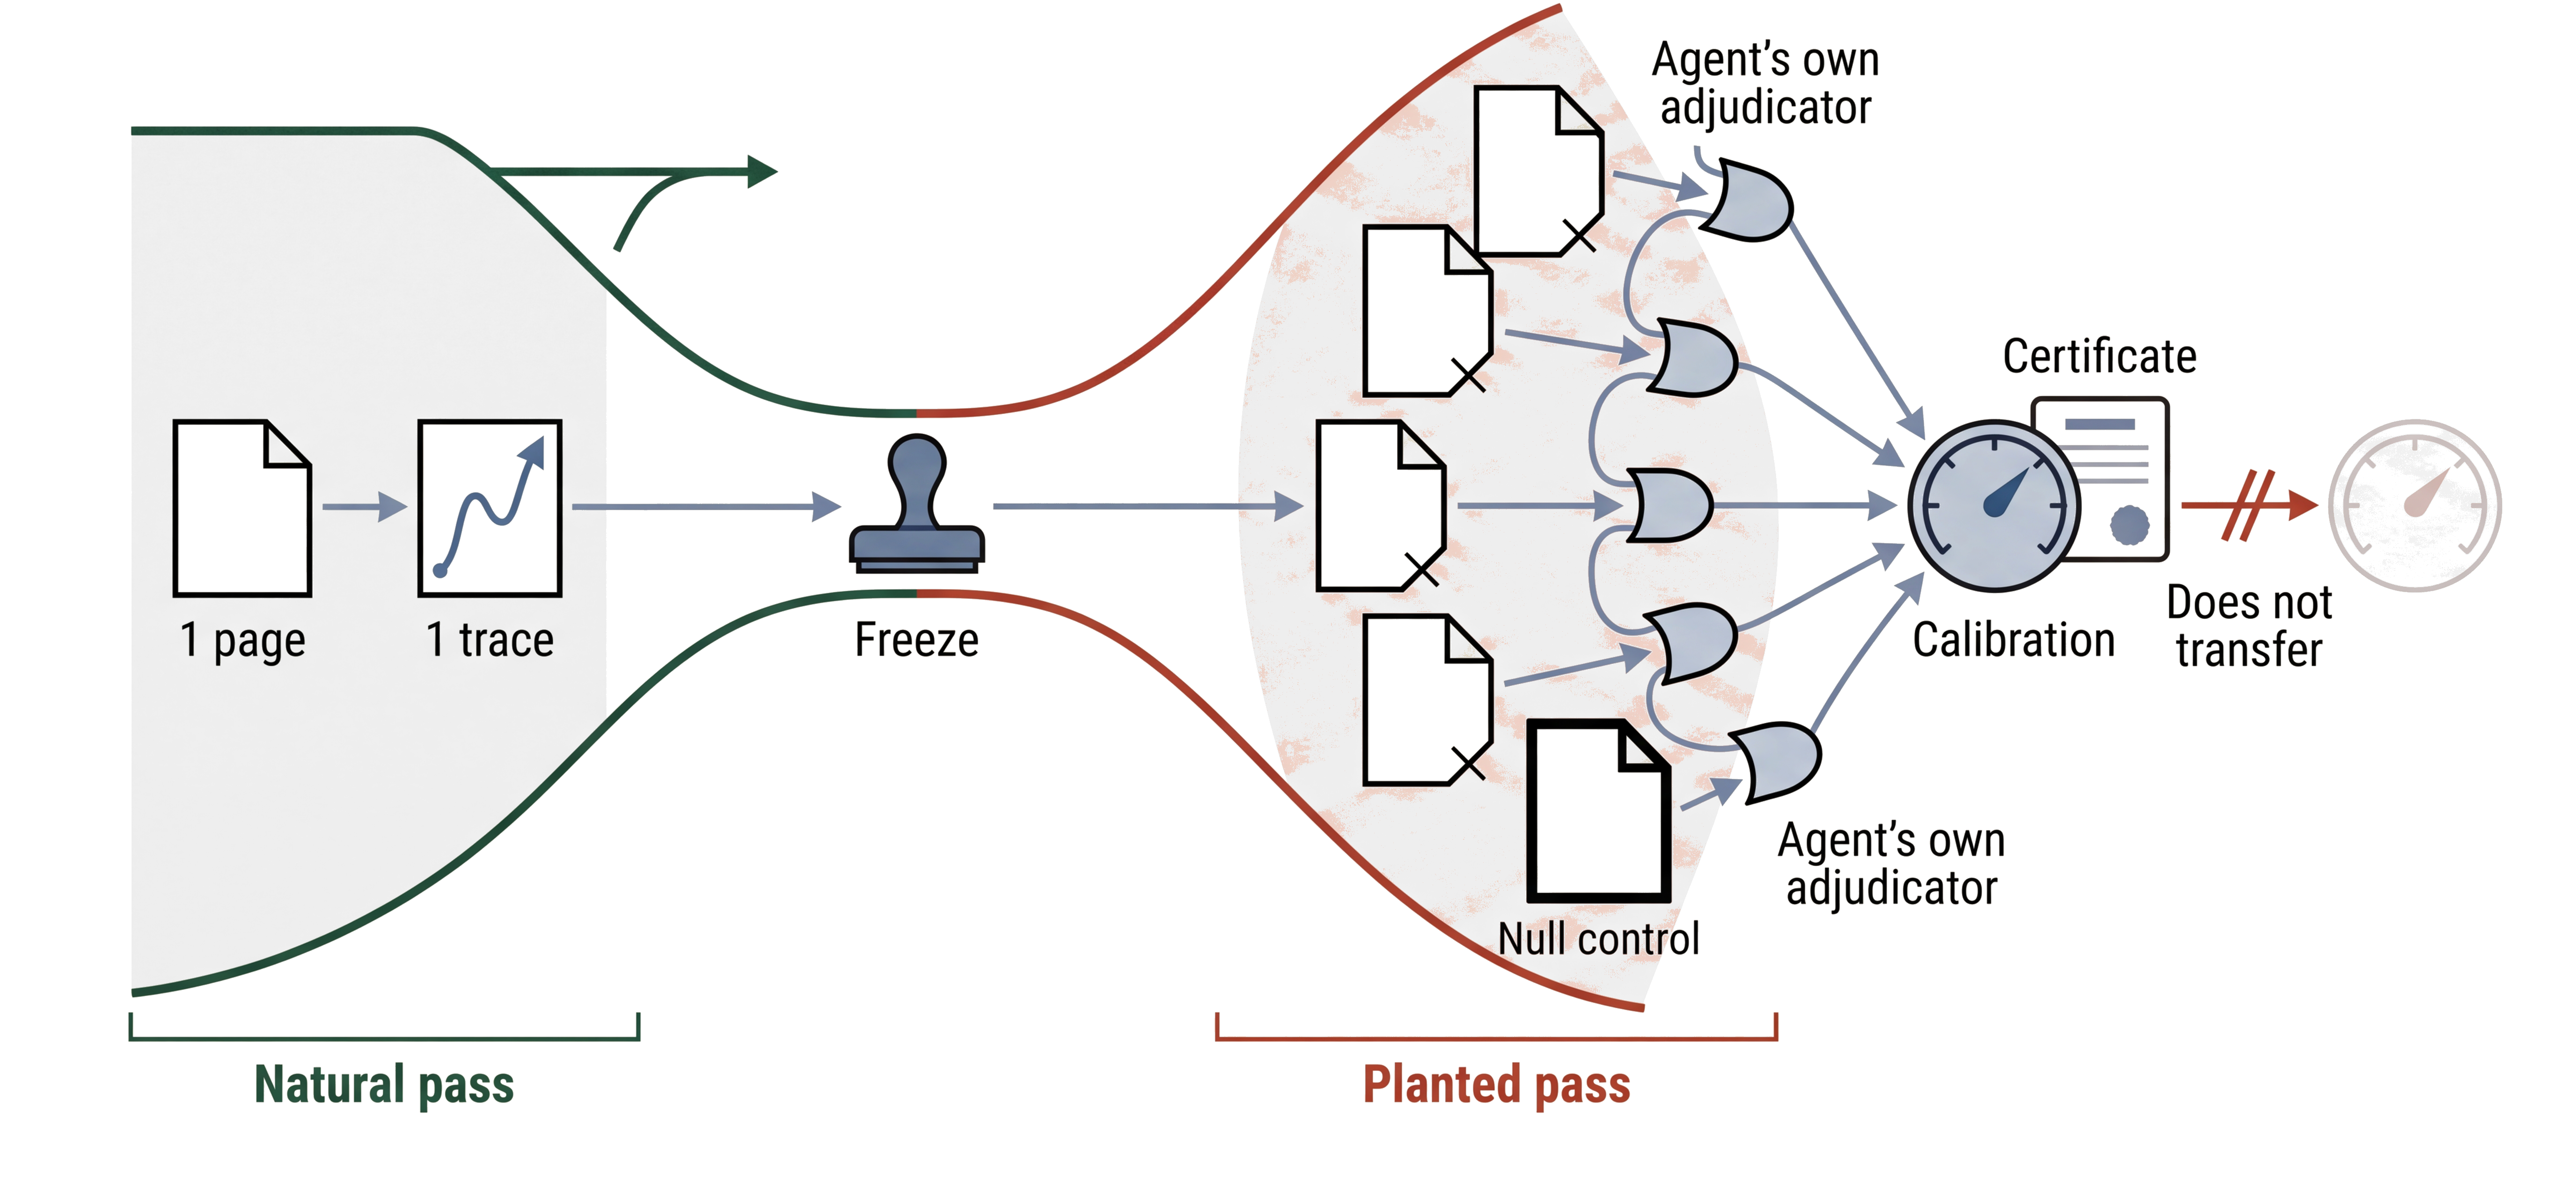
\includegraphics[width=0.82\textwidth]{figures/fig2_two_passes.png}
\caption{\textbf{The natural pass measures the agent; the planted pass calibrates the ruler.} The natural pass yields one real trace and the
process-fidelity column at no extra cost, because that same trace is the
substrate for the planted pass: the agent is never re-run. One replica has
nothing planted and must not fire. The resulting error rates belong to that
agent alone.}
\label{fig:twopasses}
\end{figure}

\subsection{The four columns, and what became of them}
Of the four columns the design calls for, only the first survives contact with
this paper's own results. They are \textbf{(1) auditable claims $N$}, how many
claims left evidence to check against; \textbf{(2) process fidelity}, how many
of those disagree with the evidence on a natural pass; \textbf{(3) self-check
credibility}, whether the agent's adjudicator catches what we planted; and
\textbf{(4) first stage to break}, columns 2 and 3 computed per stage.
Column~3 as specified is not comparable across systems, since an $e$-value
computed against a larger universe is larger for the same detection and
\S\ref{sec:e7} measures a \RM{178}-fold inflation from padding alone;
\S\ref{sec:rates} replaces it with rates that padding cannot move. Columns~2
and~4 require a universe of usable size, and \S\ref{sec:firstarm} finds \RM{2} runs in \RM{58} above the
recorded floor and none that can certify.

\subsection{Three quantities that must never be conflated}
$\Phi$ coverage is a limitation \emph{of ours}, $N$ a fact about the agent's
\emph{recording discipline}, and detection a fact about its \emph{capability};
reading the first as the second turns ``our matcher cannot parse this format''
into ``this system is unauditable'', one number supporting opposite conclusions.
Every arm reports all three side by side. Attribution is mechanical: no token
shared with any index key means the run recorded nothing on that subject and the
loss is the arm's, while candidate keys that cannot be narrowed to one make it
ours, as do declared files we could not read. On the development arm almost all of the
loss is ours: of \RM{213} unresolved claims, \RM{8} are cases where the run
recorded nothing on the subject and \RM{205} are ours, a parse-failure rate of
\RM{55.1\%} against a not-recorded rate of \RM{2.2\%}. The single figure of
\RM{42.7\%} coverage conceals exactly that split, and it conceals it in the
direction unflattering to the instrument rather than to the arm
(Appendix~\ref{app:attribution}).

\subsection{Arms and tasks}
We report \RM{five} sources across \RM{four} independent corpora, chosen by what
is publicly released with both a manuscript and its artifacts. Three came first:
AI Scientist-v2 and MLR-Agent from MLR-Bench \cite{mlrbench}, and ARA
\cite{ara} from an independent group. Two were added after those returned
nothing scoreable, to test whether that was a property of one corpus ---
AI Scientist-v1's own released papers, which ship the manuscript as LaTeX
source, and the ICML 2026 reproduction challenge, a community corpus whose
submissions carry an explicit per-claim logbook. Tasks come from that published suite rather than from us, and for the two
MLR-Bench arms they are the same ten tasks the corpus annotates for
hallucination. RH is the in-sample development arm, excluded from any ranking
claim; the extractor, the planter and every threshold are developed on it and
the external arms are only run, never tuned against, though ``our own arm'' is
one manuscript of seven (\S\ref{sec:phi}) and \S\ref{sec:limits} states what
that costs. 

\section{Results}
\label{sec:resultsec}

\subsection{Is the instrument sound?}
Before any claim about an agent, the instrument has to answer for itself: what it
buys over reading the manuscript, how much it moves when nothing else does, whether
a stronger reader would find more, and what it can resolve at all.

\subsubsection{What the artifacts buy, and what a rubric measures}
\label{sec:e4}

\textbf{The two adjudicators separate on detection, not only on significance.}
Facing the same sealed package and the same universe, the artifact-holding
adjudicator catches \RM{100\%} of planted link-breaks over \RM{12} replicates
(\RM{$\widehat{\mathrm{det}}=1.00$}, range \RM{[1.00,1.00]}) while the
manuscript-only one catches \RM{46\%} (median over \RM{4} replicates, range
\RM{[0.20,0.67]}); false accusations are \RM{0} for the first and at most
\RM{0.6\%} of unplanted bindings for the second. The corresponding $e$-values
have medians \RM{231} and \RM{11}, and a median is all they can be: each sweep
spans several planting budgets, $e$ is a steep function of $K$, and a single
figure taken across them is a summary of the sweep rather than a property of the
adjudicator. That is the second reason \S\ref{sec:rates} reports the rates ---
they are comparable across $K$ where the $e$-values are not. One sees
the frozen artifacts, one sees only the manuscript. The first recovers every
planted claim on every draw --- $A=X=K$ in all \RM{12} replicates --- so its
$e$ is a function of $K$ alone; the second recovers a variable fraction, and at
$K=\RM{3}$ its median $e$ over fresh draws is \RM{3.64} against the first's
\RM{405}. \RM{3} of its runs place accusations inside the universe while hitting
nothing planted. What separates them is a distribution, not a floor:
\S\ref{sec:variance} exhibits a draw on which the two are indistinguishable.
The negative control belongs to that second adjudicator, and it is not clean: over
\RM{5} replicates with nothing planted it accused \RM{0} slots on four and
\RM{2} on the fifth. Both are false accusations, and neither is evidence --- with
$K=0$ there is nothing to hit, so $X=0$, $p=\RM{1}$ and $e=\kappa=\RM{0.5}$ however many slots are
named. A design that could not accuse under the null would be the stronger
result; what we can report is that accusing under the null never produced one.
Appendix~\ref{app:validation} gives both sweeps and the ordering-recovery check.

\begin{figure}[t]
\centering

\includegraphics[width=0.74\textwidth]{figures/fig3_e4_axis_inversion.pdf}
\caption{Same experiment, three writers. Median movement of each rubric axis
when only the model writing the paper changes. The axes describing the
experiment move four times further than the axes describing the write-up, which
is the wrong way round, and the score carries no uncertainty against which
either movement could be judged.}
\label{fig:e4}
\end{figure}

\textbf{A published rubric is writer-dominated, and inverted.} MLR-Bench
generates three manuscripts per run from identical experiments, code and
artifacts. Under that writer swap its Overall score moves by a median of
\RM{2.0} and a maximum of \RM{3.5} on a corpus spanning 2.5--7.5, and
the axes describing the experiment --- Soundness, Significance --- move
\RM{2.0} where the axes describing the prose --- Clarity, Novelty --- move
\RM{0.5} (Figure~\ref{fig:e4}). We are not entitled to call the rubric wrong,
and neither is it: with no error bar there is no quantity against which a
movement can be judged. The fragility is not ours alone to report --- rubric
judges are independently documented to carry position bias \cite{more2026} and
to disagree with human reference in ways their own reports do not surface
\cite{when2026}. Our own $N$ moves too, disagreeing about the best
write-up on \RM{7} of \RM{10} tasks; the difference is that $N$ is declared a
property of the write-up and reported beside its denominator.

\subsubsection{Two variances, and the larger one is not the adjudicator}
\label{sec:variance}
Every external certificate here is one call to one adjudicator on one sealed
package, and two different things can move under resampling: the adjudicator,
and the draw. We separated them. Holding one package byte-identical and
adjudicating it \RM{6} times isolates the first; drawing a fresh planted set for
each of \RM{5} replicates, same substrate, same $K$, same concealment and the
same model, isolates the second.

\begin{center}
\small
\begin{tabular}{@{}lccc@{}}
\toprule
same model, same substrate, $K=\RM{3}$, $\delta=\RM{0.30}$ & hits $X$ & $e$ & certifies \\
\midrule
one package, adjudicated \RM{6} times   & \RM{2}--\RM{3} & \RM{32.4}--\RM{405} & \RM{6/6} \\
fresh planting each replicate           & \RM{0}--\RM{2} & \RM{0.5}--\RM{32.4}  & \RM{2/5} \\
\midrule
\emph{that same package}, artifact-holding adjudicator & \RM{3} & \RM{405} & \RM{1/1} \\
\bottomrule
\end{tabular}
\end{center}

\noindent \textbf{The draw moves the answer more than the adjudicator does.}
Resampling the adjudicator on fixed bytes leaves the decision intact --- all
\RM{6} calls certify --- while moving $e$ over a \RM{12.5}-fold range. Redrawing
the planted set flips the decision itself: \RM{2} of \RM{5} replicates certify
and \RM{3} do not, on the same substrate against the same model. Which slots
happen to be planted matters more than which call adjudicates them.

\noindent \textbf{On this draw the two adjudicators are the same instrument.}
The third row is the matched control the first two require: the artifact-holding
adjudicator, run on the identical bytes. It recovers \RM{3} of \RM{3} at
$e=\RM{405}$ --- which is the median of the manuscript-only reader's six calls on
those same bytes. The M2/M1 $e$-ratio on this matched draw is \RM{1.00}
(\texttt{e21.py}), against the unmatched separation of \S\ref{sec:e4} where the
same two adjudicators differ by two orders of magnitude across fresh plantings.
This is the sharpest form of the preceding paragraph and we state it against
ourselves: the fixed package is a \emph{favourable} draw, one whose planted
claims are visible without the artifacts, and on it the reader we describe as
handicapped is not. Nothing about the design prevents that. A single planting
does not order the two adjudicators, and no claim in this paper may rest on one.

That has a consequence for every single-shot certificate in this paper, and it
is not the consequence we first drew. An earlier revision reported the
fixed-package result alone and concluded that the binary outcome is robust to
resampling. It is robust to resampling \emph{the adjudicator}; it is not robust
to resampling \emph{the draw}, and the second is the randomness the design
actually depends on. A certificate from one planting is a sample of size one
from the distribution that matters.

It is also why \S\ref{sec:rates} reports rates with the $e$-value as a
significance guard rather than as a score, and why \S\ref{sec:power} bounds what
$K=\RM{3}$ can resolve at all: at that budget the hit count is one of four
values, so a single draw carries very little.

\subsubsection{Is it the matcher? A ceiling estimate says no}
\label{sec:ceiling}
Our matcher is a frame-overlap heuristic with published thresholds, so the
negative result is unbounded until something stronger is tried on the same
inputs. We give a frontier model the manuscript and the same list of artifact
keys the frozen contract admits, ask it for cell-level bindings, and then verify
every binding it proposes against the index: a binding counts only if the key
exists and the cited value matches that cell to the printed precision.

\begin{center}
\small
\begin{tabular}{@{}lrrr@{}}
\toprule
over \RM{10} AI Scientist-v2 tasks & median & max & runs reaching $N \ge \RM{23}$ \\
\midrule
our matcher                & \RM{2}   & \RM{5} & \RM{0} \\
model bindings proposed    & \RM{5}   & \RM{16} & \RM{0} \\
model bindings \emph{verified} & \RM{1.5} & \RM{5} & \RM{0} \\
\bottomrule
\end{tabular}
\end{center}

\noindent \textbf{The stronger extractor does not clear the floor either.} It
beats our matcher on \RM{4} of \RM{10} tasks and trails on the rest, for a
verified median of \RM{1.5} against our \RM{2} --- so it is not uniformly worse,
and the comparison that matters is not with us but with the floor: its best task
reaches \RM{5} where evidence requires \RM{23}. The model was given the complete
key index for every task; an earlier run of this experiment sampled \RM{400}
keys and withheld two thirds of them from the three largest tasks, which is a
handicap the ceiling exists to avoid. The gap between proposed and verified is where it fails, and
it fails in the way \S\ref{sec:e5} predicts: the model never invented a key
--- \RM{0} proposed keys were absent from the index --- but the values it cited
did not match the cells it named. Asked to bind claims to cells, a strong reader
of an unmarked manuscript falls back on matching numerals, which is the
procedure the acceptance test rules out.

\textbf{This is a ceiling, not a pipeline, and it is not reproducible.} One task
returned \RM{6} verified bindings on one call and \RM{0} on another with the
same inputs. A quantity that moves like that cannot be frozen, cannot be
pre-registered, and cannot carry a certificate; it can only bound how much a
better matcher would recover, and the bound it gives is below what we already
recover. The claim that the information is absent rather than merely missed is
supported to that extent and no further.

\subsubsection{What the design could have detected, and what it cost}
\label{sec:power}
Saying a design lacked power is an admission; a bound is a number. Under the
planted null a universe of size $N$ with $K$ planted slots and an adjudicator
catching a fraction $q$ of them yields $e = \kappa\,p^{\kappa-1}$ with
$p = \Pr[\mathrm{Hyp}(N,K,A)\ge \lceil qK \rceil]$, so the smallest $q$ the
design separates from chance follows from $N$, $K$ and the replicate count.

\begin{center}
\small
\begin{tabular}{@{}lrrrr@{}}
\toprule
planted per replicate & \RM{1} rep & \RM{3} reps & \RM{5} reps & \RM{20} reps \\
\midrule
$K=\RM{3}$ \emph{(this paper's sweep)} & \RM{50\%} & \RM{17\%} & \RM{17\%} & \RM{17\%} \\
$K=\RM{5}$   & \RM{51\%} & \RM{11\%} & \RM{11\%} & \RM{11\%} \\
$K=\RM{10}$  & \RM{26\%} & \RM{15\%} & \RM{6\%}  & \RM{6\%}  \\
\bottomrule
\end{tabular}
\end{center}

\noindent \textbf{Past three replicates, under the deterministic rule used here,
resolution is bought with planting budget and not with runs.} With $K=\RM{3}$ the
hit count is one of $\{0,1,2,3\}$, so under the calculation that sets
$X=\lceil qK\rceil$ per replicate the bar falls from \RM{50\%} at one replicate
to \RM{17\%} at three and then stops, unchanged at \RM{20}. That plateau is a
property of this rule, not an information-theoretic limit: a stochastic analysis
of the frequency of hits across replicates can resolve detection probabilities
below one third. Where $K$ is larger the same deterministic rule keeps paying
with replicates for longer: at $K=\RM{10}$ the bar falls \RM{26\%}, \RM{15\%},
\RM{6\%} across one, three and five replicates. The table is computed at the
development $N=\RM{159}$ and $\alpha=\RM{0.05}$; it is a minimum-detectable-$q$
chart under that rule, not a Monte-Carlo power curve. Our concealment sweep used $K=\RM{3}$ with \RM{5} replicates, which means
it could only ever resolve ``catches at least one of three''. Reporting that M1
does not certify at any concealment level therefore says M1 did not reliably
reach even that, and it says nothing finer. At $K=\RM{10}$ and the same
replicate count the bar would be \RM{6\%}. This is a design fact we should have
derived before the sweep rather than after it.

\paragraph{Cost.} The construction's premise is that adjudication, not
planting, is the scarce resource, and that had not been priced. Every
certificate line in this paper costs one adjudication and there are \RM{146} of
them: \RM{12} for the artifact-holding sweep, \RM{6} plus \RM{34} plus a
\RM{10}-call re-measurement for the manuscript-only sweeps, \RM{20} for the
ordering-recovery check, \RM{6} for the fixed-package replicates, and one for
each of the \RM{58} external runs. That is the audit's price, not the paper's:
the ceiling estimate and the two writer experiments also call a model, and
folding them in would price the audit using calls the audit does not make. The
deterministic stages around them cost
\RM{0.4}\,s on the development substrate: \RM{0.01}\,s to build a
\RM{3430}-key artifact index and \RM{0.36}\,s to extract the universe. For
contrast, the arm we audit spent a median of \$\RM{1.85} and
\RM{1{,}068{,}286} tokens \emph{producing} each run, by its own ledger. The
premise holds, but one-sidedly: our own adjudicator's token spend was not
recorded at the time and we do not reconstruct it.

\subsection{What the released corpora yield}
With the instrument bounded, we turn it on what has been released.

\subsubsection{The validity domain, measured}
\label{sec:firstarm}

\begin{table}[t]
\centering\small
\begin{tabular}{@{}llllc@{}}
\toprule
arm & corpus & claim side & artifact side & scoreable \\
\midrule
RH \emph{(development)} & own & macro table, \textbf{cell-level} & structured tables & \RM{1 of 7} \\
AI Scientist-v2 & MLR-Bench & PDF, unmarked & source string & \RM{0/10} \\
MLR-Agent & MLR-Bench & Markdown & Markdown tables & \RM{1/30} \\
ARA & ARA-Labs & claims file, \emph{file}-level link & Markdown tables & \RM{0/3} \\
AI Scientist-v1 & own release & \textbf{LaTeX source} & nested JSON summaries & \RM{1/10} \\
ICML-26 repro challenge & community & \textbf{per-claim pages} & whatever was published & \RM{0/5} \\
\bottomrule
\end{tabular}
\caption{\textbf{Five sources across four independent corpora, and the seven
same-generator development substrates.} The claim-side column is the one that
moves the outcome: the arms with cell-level identity are the only ones that
resolve a universe at all, and even they resolve one manuscript in seven.}
\label{tab:arms}
\end{table}

Table~\ref{tab:arms} is the paper's central measurement: of \RM{58} released
external runs across \RM{five} sources and \RM{four} corpora, \RM{2} clear the
recorded floor and \RM{0} can certify under a single planting at any $K$
(\S\ref{sec:floor}). AI Scientist-v2 records its settings only
inside a source string --- median $N=\RM{2}$, parse failure \RM{95.2\%} at the median, and
by \S\ref{sec:board}'s own rule that attribution is ours. MLR-Agent, same corpus
and tasks but results written as tables, reaches median $N=\RM{3}$ and a maximum
of \RM{10}, and is one of two arms with a run above the
floor at all, the other being AI Scientist-v1 at $N=\RM{12}$. The recording contract is
measurable on identical capture, but the effect is a factor of \RM{1.5} at the
median and \RM{2} at the maximum --- too small to carry the argument on its
own. ARA is the independent source and the
constructive case --- purpose-built for auditing, shipping an explicit claim
listing, and still \RM{0/3}.

\textbf{Zero scoreable is not zero performance, and the failures are not one
failure.} Splitting every unresolved claim by cause separates arms that our
instrument cannot read from arms whose run did not record the subject at all:

\begin{center}
\small
\begin{tabular}{@{}lrrrrr@{}}
\toprule
arm & runs & no candidate & ambiguous & parse failure & not recorded \\
 & & & & \footnotesize(runs with keys) & \\
\midrule
AI Scientist-v2 & \RM{10} & \RM{3}    & \RM{436} & \RM{95.2\%} & \RM{0.0\%} \\
MLR-Agent       & \RM{30} & \RM{1200} & \RM{838} & \RM{43.4\%} & \RM{54.6\%} \\
ARA             & \RM{3}  & \RM{59}   & \RM{50}  & \RM{58.8\%} & \RM{100\%} \\
AI Scientist-v1 & \RM{10} & \RM{541}  & \RM{136} & \RM{9.2\%}  & \RM{90.8\%} \\
ICML-26 repro   & \RM{5}  & \RM{1793} & \RM{62}  & \RM{45.3\%} & \RM{100\%} \\
\bottomrule
\end{tabular}
\end{center}

\noindent The parse-failure column is taken over the runs that recorded any
artifact key at all, which is not the same as over all runs, and the difference
is not cosmetic. A run that recorded nothing has no denominator: our parser
cannot fail on a key list of length \RM{0}, and reporting that as a rate of
\RM{0\%} credits the instrument for a case it never faced. On the two arms where
most runs recorded nothing --- ARA and the ICML-26 corpus --- the median over
all runs is \RM{0.0\%} and the rate on the runs that could be parsed is
\RM{58.8\%} and \RM{45.3\%}. We report the second. The same vacuity is why
\S\ref{sec:floor} refuses to read an unscoreable run as a low error rate: an
empty denominator flatters whoever is holding it.

\noindent The two ends of that table are opposite failures. On AI Scientist-v2
the run does hold something on almost every subject a claim names --- only
\RM{3} claims find no candidate key at all --- and the loss is ours, which the
\RM{95.2\%} parse failure states directly. On ARA the run records almost
nothing: \RM{100\%} of its unresolved claims name a subject with no record,
and our parser only gets a denominator on the single run that published
artifacts. Reporting these \RM{5} arms as a single count of zero would hide that
the instrument and the substrate fail in different places, and
\S\ref{sec:board}'s rule against conflating $\Phi$ coverage with $N$ exists to
keep them apart.

\textbf{What a parse failure is, concretely.} The rate is not an abstraction
about formats. Made conjunctive to match its own stated contract --- name the
quantity \emph{and} say which record --- the binding rule leaves \RM{1} of
\RM{30} MLR-Agent runs scoreable, and inspecting the values shows the loss is
claim-side rather than binding-side: a printed \RM{4} resolving to an $F_1$ of
\RM{0.0} is a section number, and a printed \RM{2018} is a citation year. On
\LaTeX{} the extractor separates assertions from prose numerals because the
source marks them --- plumbing commands are stripped, tables are read by column
spec. Markdown and PDF carry no such marking, and no cue list we are willing to
defend recovers it.

The attribution is conservative in one direction, and deliberately so. Our
matcher fails on AI Scientist-v2 because that arm's results are prose in a PDF,
so the \RM{95.2\%} charged to us is itself downstream of the missing claim
marking; a rule that followed the causal chain would charge much of it to the
arm. We keep the mechanical rule because the alternative lets an evaluator
attribute its own parsing limits to whatever it is evaluating, and \S\ref{sec:limits}
records that a better matcher would raise every $N$ here. None of this says the
underlying research is wrong: an unscoreable record supports no error rate,
high or low.

\textbf{The development side is one manuscript of seven.} Under a fixed
generator, format and pipeline, $N$ is \RM{159} on one substrate and
\RM{$\leq$4} on the other six, with every failing declaration matching its files
(\S\ref{sec:phi}). Whether a claim binds is a property of how a manuscript
happens to be phrased, not of the pipeline that wrote it.

\subsubsection{The floor is derivable, and the one we froze was too low}
\label{sec:floor}
A count of runs above a threshold is worth only as much as the threshold, so we
sweep it. The count moves: \RM{32} of \RM{58} external runs clear a floor of
\RM{2}, \RM{12} clear \RM{5}, \RM{2} clear the frozen \RM{10}, and \RM{0} clear
\RM{20}. The headline therefore cannot be defended by saying the threshold does
not matter. What defends it is the freeze --- the floor was fixed before any
external arm was run and the manifest timestamps it --- and the derivation
below, which says the value we froze was the wrong one.

\begin{center}
\small
\begin{tabular}{@{}lrrrrr@{}}
\toprule
& \multicolumn{5}{c}{most evidence attainable, $e^{\max}$} \\
\cmidrule(l){2-6}
universe size $N$ & $K{=}1$ & $K{=}2$ & $K{=}3$ & $K{=}5$ & external runs at least this large \\
\midrule
\RM{5}   & \RM{1.1} & \RM{1.6}  & \RM{1.6}  & ---        & \RM{12} \\
\RM{10}  & \RM{1.6} & \RM{3.4}  & \RM{5.5}  & \RM{7.9}   & \RM{2}  \\
\RM{23}  & \RM{2.4} & \RM{8.0}  & \RM{21.0} & \RM{91.7}  & \RM{0}  \\
\RM{159} & \RM{6.3} & \RM{56.0} & \RM{405}  & \RM{14096} & \RM{0}  \\
\bottomrule
\end{tabular}
\end{center}

\noindent A universe of size $N$ with $K$ planted slots cannot yield more than
$e^{\max} = \kappa\binom{N}{K}^{1-\kappa}$, attained when the adjudicator
accuses exactly the planted set and nothing else. A single stratum needs
$e \ge 1/\alpha = \RM{20}$. At the frozen floor of $N=\RM{10}$ with $K=\RM{3}$
the ceiling is \RM{5.5}, so a run sitting exactly on that floor \emph{cannot
produce a certificate even against a perfect adjudicator}. $K=\RM{1}$ is the
worst case: $e^{\max}=\kappa\sqrt{N}$ there, so it needs $N\ge\RM{1600}$ ---
finite, and two orders of magnitude beyond anything released. The smallest universe that can
certify at $K=\RM{3}$ is $N=\RM{23}$.

\textbf{So the external count is \RM{0}, not \RM{2}.} The two runs that
clear the recorded floor clear a floor set below the point where evidence
becomes attainable. We report the frozen value because it is what was frozen and
this derivation because it is what the frozen value should have been; a floor
chosen after seeing the arms would have been worth nothing either way.

\subsubsection{A community corpus exhibiting three distinct failure modes}
\label{sec:e19}
The four agent arms are four releases by four teams. The fifth corpus is not:
the ICML 2026 agent reproduction challenge asks participants to publish a
workspace of scripts, configs, outputs and logs alongside a logbook that
indexes one page per claim. That logbook is a face-C implementation in the
wild, so this is a second chance to consume one rather than describe it, and
the artifact side is mandated rather than incidental.

Of \RM{51} submitted logbooks, \RM{5} published machine-readable results at
all; of \RM{18} sampled the rest, every one shipped an empty traces index. The
\RM{5} that did publish fail in three distinct ways:

\begin{center}
\small
\begin{tabular}{@{}llll@{}}
\toprule
submission & claim side & artifact side & missing \\
\midrule
mp-moe            & claim pages & \RM{22} cells   & --- ($N=\RM{1}$) \\
last-iterate      & \textbf{none}        & \RM{47} cells   & face C \\
gaussian-mechanism & claim pages & trace log only  & face B \\
learning-to-share  & claim pages & trace log only  & face B \\
success-conditioning & claim pages & CSV, no row labels & cell identity \\
\bottomrule
\end{tabular}
\end{center}

\noindent \textbf{The faces fail independently, and all three modes appear in
five submissions.} One published a summary with \RM{47} addressable cells and no
claim pages; two published execution traces rather than result records, so there
is nothing to bind \emph{to}; one published a CSV whose columns are all numeric,
which has values but no addressable cells --- a row with no label has no stable
name for a claim to point at, which is the same requirement \S\ref{sec:three_faces}
states from the other side. Only one submission has both sides, and it binds
$N=\RM{1}$.

This corpus matters because the artifact side was \emph{required} here. Where an
agent release omits records by default, these participants were asked for them
and the omission survived the asking. That is evidence the gap is not a
property of any one system's engineering.

\subsubsection{The hierarchy is unexercisable on every substrate we measured}
\label{sec:e11}
The tree the sequential test acts on is a containment hierarchy, and on the
development substrate it has one usable node. Of \RM{159} bound slots,
\RM{144} sit in a single record and the remaining \RM{15} are spread over
\RM{10} containers, nine of which hold exactly \RM{1}; a
node with one slot cannot carry a hypergeometric test, so the effective depth is
one. The table-recording external arm is the same shape at smaller scale:
\RM{10} slots over \RM{4} containers, sized \RM{[7,1,1,1]}.

\textbf{That collapse is a property of citation, not of artifacts.} The same run
holds \RM{50} containers, \RM{6} of them with more than twenty numeric cells.
The manuscript simply draws almost everything from one summary record. So the
recording contract has a fourth consequence we had not stated: it fixes not only
whether claims can be checked but the resolution at which they can be
\emph{localised}. A run that flattens its results into one table is auditable
and unlocalisable, and column~4 is unavailable for a recording reason rather
than a statistical one.

\textbf{A structure-preserving writer restores the tree, and sequential
stopping is what the tree returns.} Constraining the reference generator of
\S\ref{sec:e10} not to draw every value from one record --- which costs the
writer nothing at write time --- yields \RM{3} usable nodes of \RM{14} slots
each. On that substrate the artifact-holding adjudicator certifies after
\RM{2} replicates rather than a fixed budget, and each replicate not spent is
one adjudication of a sealed package.

\begin{center}
\small
\begin{tabular}{@{}lrr@{}}
\toprule
adjudicator & stateless stop & stateful stop \\
\midrule
\textbf{M2, artifact-holding (measured)} & $n=\RM{\textbf{2}}$ & --- \\
\midrule
\multicolumn{3}{@{}l}{\emph{parametric sweep, detection rate $q$}} \\
$q=1.0$ & $n=\RM{2}$  & $n=\RM{3}$ \\
$q=0.5$ & $n=\RM{4}$  & none in \RM{20} \\
$q=0.2$ & none in \RM{20} & none in \RM{20} \\
$q=0.0$ & none in \RM{20} & none in \RM{20} \\
\bottomrule
\end{tabular}
\end{center}

\noindent Only the first row is measured; the sweep varies a detection rate we
supply, and is here to show the ordering and the negative control rather than
to report a system. The blind adjudicator never fires.

\textbf{The stateful column cannot be read as a comparison.} Under a stateful
adjudicator Proposition~A does not apply, so those stopping times carry no
anytime guarantee at all. We print them because they look unremarkable: nothing
in the output distinguishes a run whose guarantee holds from one whose guarantee
is void, which is precisely why statelessness has to be enforced and recorded in
the freeze manifest rather than inferred from results.

\subsection{What would fix it}
A negative result is only useful if something would change it. Four routes fail and
one works, and the one that works is available to a writer that is not ours.

\subsubsection{Necessity, and then sufficiency}
\label{sec:e5}

Four independent routes fail without cell-level claim marking, and each fails
differently. Patching the artifact side leaves \RM{0/10} scoreable and does not move the
median at all --- \RM{2.5} before and after, with \RM{2} of \RM{10} tasks
changing by one claim (\S\ref{sec:e5}). Retrofitting the claim side
from printed values yields \RM{25} marks against the matcher's \RM{2} --- enough
to clear the floor --- and then fails the acceptance test, because planting a
value removes its slot from the universe and the certificate is computed against
different objects before and after. Consuming ARA's claim-to-table pointer drops
$N$ from \RM{1} to \RM{0}. And a macro table, which all seven development
substrates ship, binds \RM{0--17\%} of its macros, supplying a stable
\emph{name} where the denominator needs a \emph{pointer}.
Appendix~\ref{app:extended} gives each.

\begin{figure}[t]
\centering

\includegraphics[width=0.74\textwidth]{figures/fig4_e7_padding.pdf}
\caption{Padding the universe with trivially checkable claims while holding the
adjudicator's measured behaviour fixed. The $e$-value rises without a single
additional planted claim being caught. The test is behaving correctly; the
leaderboard column that compares such values across arms is not.}
\label{fig:e7}
\end{figure}

\textbf{Our own proposed column is inflatable, and no lie is required.}
\label{sec:e7}
Holding $K$, $A$ and $X$ at the development arm's measured line, padding $N$ from
\RM{159} to \RM{2412} multiplies $e$ by \RM{60} and to \RM{5000} by \RM{178}
(Figure~\ref{fig:e7}). The test is not wrong --- a larger universe does make the
same hits less likely by chance --- but comparing $e$-values computed against
universes of different sizes is, and that specification is ours. Column~3 needs
a size-invariant estimate with the $e$-value kept as a significance guard.

\textbf{The preregistered cross-benchmark test voids, and which condition fired
matters.} Of \RM{10} released runs \RM{0} clear the floor, so the non-evaluable
fraction is \RM{100\%} against a threshold of \RM{30\%} fixed in advance, and we
report VOID rather than support or contradiction. The registration's second condition voids if our
parse failure exceeds twice the development arm's, which the freeze records as
\RM{55.1\%}, so the threshold is \RM{110.2\%}. A parse-failure rate cannot
exceed \RM{100\%}, so that condition could not have fired however the audit went;
we report it as the vacuous guard it was rather than as discipline it was not
(Appendix~\ref{app:e8}).

\subsubsection{Sufficiency: a reference-compliant generator}
\label{sec:e10}
Necessity can be measured on corpora that do not comply; sufficiency needs a
reference implementation. A generator that emits the artifact key alongside each
reported value produces a substrate on which all \RM{40} emitted claims resolve
(\RM{100\%}, against \RM{0--44\%} without), the slot-name set is invariant under
planting, the certificate returns $A=X=K=\RM{3}$ at $e=\RM{49.7}$, and the
negative control accuses \RM{0} --- every check that fails elsewhere passes. Its
manuscript is plain prose, one sentence per value, with values read from a real
run and the writing ours, so this states what the pointer buys once it exists,
not that agents will supply it. That gap is the engineering this paper asks for
rather than reports.

\subsubsection{A writer that is not ours can meet the contract}
\label{sec:e17}
The generators of \S\ref{sec:e10} and \S\ref{sec:e11} are ours, so they show
what the contract buys once met and not that anything but a Python loop can meet
it. We therefore gave a frontier model a real run's artifact cells and asked it
to write a results section \emph{under the contract}: print no number you cannot
key, and emit the key beside it. Its marking is then audited exactly as any
arm's would be.

\begin{center}
\small
\begin{tabular}{@{}lrr@{}}
\toprule
same model, same artifacts, the \RM{5} tasks of this run & median per task & total \\
\midrule
asked to \emph{recover} marking from unmarked prose (\S\ref{sec:ceiling}) & \RM{1} & \RM{6} \\
asked to \emph{emit} marking while writing & \RM{17} & \RM{96} \\
\midrule
of those emitted: key resolves in the index & \multicolumn{2}{c}{\RM{96/96}} \\
value printed in the prose it wrote & \multicolumn{2}{c}{\RM{96/96}} \\
value matches the cell named & \multicolumn{2}{c}{\RM{96/96}} \\
\bottomrule
\end{tabular}
\end{center}

\noindent \textbf{The same model, the same information, an order of magnitude
apart.} Over these five tasks the recovery arm verifies \RM{6} bindings and the
emission arm \RM{96}. The only difference is when the marking is written. Recovering it
afterwards leaves the model matching numerals, which \S\ref{sec:e5} shows the
acceptance test forbids; emitting it while writing adds only the tokens of the
key itself, which is already in front of the writer, and caused no measured loss
in binding coverage. Every one of the \RM{96} bindings it
emitted survived the audit --- the key resolved, the value appeared in its
prose, and the value matched the cell.

\textbf{And these universes can certify.} By \S\ref{sec:power}, $N=\RM{17}$
reaches $1/\alpha$ at a planting budget of $K\ge\RM{4}$ and $N=\RM{23}$ at
$K\ge\RM{3}$; all \RM{5} tasks clear their own bar at some $K$. No released run
clears it at any $K$. The contract is therefore satisfiable by a writer that is
not ours, and satisfying it is what moves a substrate from uncertifiable to
certifiable.

\subsubsection{The agent's own instruction, with and without the clause}
\label{sec:e18}
The objection to \S\ref{sec:e17} is that the instructions were ours. So we took
AI Scientist-v1's own Results-section instruction verbatim from its writeup
code and changed exactly one thing: whether the recording-contract clause is
appended. Same artifacts, same model, same everything else.

\textbf{That instruction already demands truthfulness.} It says, in the agent's
own words, ``Only includes results that have actually been run and saved in the
logs. Do not hallucinate results that don't exist.'' The papers released under
it bind a median of \RM{0} claims. Instructing a writer not to fabricate does
not make its output auditable, because fabrication is about values and
auditability is about pointers.

\begin{center}
\small
\begin{tabular}{@{}lrrr@{}}
\toprule
artifact cells available & \RM{16} & \RM{28--40} & \RM{48} \\
\midrule
agent's tip verbatim, bound by value matching & \RM{16} & \RM{24}, \RM{2} & \RM{4} \\
agent's tip $+$ contract clause, bound        & \RM{16} & \RM{28}, \RM{40} & \RM{48} \\
\bottomrule
\end{tabular}
\end{center}

\noindent \textbf{The clause is free at \RM{16} cells and decisive at \RM{48}.}
These are different papers, not controlled enlargements of one index, so the
comparison is an association across artifact sizes rather than a causal effect of
size alone. With a small index almost every printed numeral matches exactly one
cell, so value matching recovers everything and the clause changes nothing. At
the larger indexes value matching collapses --- \RM{2} of \RM{40}, \RM{4} of
\RM{48} --- while the marked arm binds every cell it was given, at every size. The retrofit that \S\ref{sec:e5} rules out on principle therefore
also fails in practice, and it fails exactly where it would start to matter:
a universe small enough for value matching to work is a universe too small to
certify (\S\ref{sec:floor}).

\textbf{What this comparison is and is not.} Control and treatment differ by one
clause and nothing else, so the difference between them is attributable. The
sweep covers \RM{6} papers and the table reports \RM{5}: on
\texttt{dual\_expert\_denoiser} both arms bind \RM{0} because the run published
no artifact cells, so the clause has nothing to act on and the pair carries no
information about it. We name it rather than drop it silently, for the reason
\S\ref{sec:firstarm} gives about empty denominators. Neither
is comparable to the released papers: those were written by the full agent with
citations, figures and iterative refinement, and the median of \RM{0} they bind
reflects that whole pipeline rather than this instruction alone. The claim here
is narrow --- adding the clause to the agent's own instruction changes what
binds, and the change grows with the size of the universe at stake.

\section{Discussion and limitations}
\label{sec:limits}

\textbf{We speak only about the mechanically checkable subset.} Whether the idea
is good, the method appropriate or the writing clear we do not say, and those
are exactly what rubric benchmarks do say. On our development arm $\Phi$
coverage is \RM{42.7\%}, and of what does not resolve, \RM{205} of \RM{213}
cases are our matcher rather than the arm's record. Most of the manuscript is
invisible to us, and that is our limitation. Process fidelity is a precondition
rather than another axis --- a system scoring well on a quality leaderboard
while reporting untrustworthy numbers has an uninterpretable score --- so we do
not replace those benchmarks but supply the condition under which their numbers
mean something.

\textbf{The assertion catalogue is anchored in two machine-learning reporting
standards.} Cross-disciplinary arms need their field's own standards, and no
cross-disciplinary conclusion may be drawn until that is done.

\textbf{The positive results rest on one substrate selected, after the fact,
from seven.} Every threshold and matching rule was tuned on the single
same-generator manuscript where a usable universe resolves; the other six yield
$N \leq 4$, and we do not know what makes it different. Until we do, every
positive certificate in this paper is a claim about one manuscript, not a
pipeline --- and even on that manuscript the construction yields a universe only
when the draw cooperates (\S\ref{sec:variance}). One model and five replicates
per level compound this: we report that M1 does not certify at any concealment
level tested, but at this power we could not resolve a threshold if one existed,
and that must not be read as establishing its absence.

\textbf{The negative result could be our instrument rather than their
recording, and that is the primary threat.} Three measurements separate the
readings. The same extractor on the same tasks returns median $N=\RM{2}$ against
manuscripts whose results live in a source string and median $N=\RM{3}$ against
manuscripts whose results live in tables --- a difference in the arms, since
nothing on our side changed, though a factor of \RM{1.5} is weak taken alone; the instrument separates an artifact-holding adjudicator
from a manuscript-only one by two orders of magnitude
(Appendix~\ref{app:validation}), so it is not inert; and a generator built to
comply makes \RM{40} of \RM{40} claims resolve, so the failures are not a
ceiling of the method. A better matcher is the obvious remaining explanation, and
\S\ref{sec:ceiling} bounds it: a frontier model given the same inputs verifies
a median of \RM{1.5} bindings against our \RM{2}, beating our matcher on
\RM{4} of \RM{10} tasks, tying on \RM{3} and trailing on \RM{3}. Its best task
verifies \RM{5}, which is half the recorded floor and less than a quarter of
the \RM{23} a universe needs to carry evidence at $K=\RM{3}$. We defend that the information is absent to that
bound, and no further --- a reader who believes a different extractor would
find it is asking for an experiment we ran and reported.

\textbf{The column we propose is not yet safe to publish as specified.} Padding
the universe with trivially checkable claims multiplies the certificate by
\RM{178} without catching one additional planted defect, and nothing in that
attack requires an arm to lie. Any leaderboard built on the $e$-value as
specified here would reward universe inflation. The fix --- a size-invariant
estimate with the $e$-value retained as a significance guard --- is stated in
\S\ref{sec:resultsec} and not implemented, so the four-column board this
construction is meant to support remains a design rather than a result.

\textbf{The construction applies to agents that record results as data.} We
designed for calibration not transferring between agents; \S\ref{sec:firstarm}
shows the boundary is sharper and sits elsewhere --- against a substrate
recording results as a source-code string the extractor returns nothing
scoreable, against one recording the same results as a table it yields a
universe --- though still not one large enough to certify. This bounds what the
construction covers, and it is
the same condition the recording contract states from the other side: what the
evaluator cannot read is what the agent did not mark.

\section{Conclusion}
An agent's own gate decides what ships, and it has never been measured; public
benchmarks measure the output and not the gate. We built the missing quantity
and then measured what it costs.

\textbf{The cost is a property of how a manuscript is written, not of how it is
evaluated.} A denominator needs to know which artifact cell each printed number
reports, and that is the one requirement no evaluation protocol can supply for
itself: an unmarked manuscript offers only the value, and a universe derived
from values dissolves under the planting it is supposed to withstand. Across \RM{58} released runs, five sources and four independent
corpora, no arm marks its claims at cell granularity --- including the corpus
purpose-built for auditing, which marks them at file granularity instead. The
failures are not interchangeable: \S\ref{sec:firstarm} separates the arm whose
record our matcher cannot read from the arm whose run did not record the
subject.

\textbf{Two findings survive without any of this being adopted.} A published
rubric moves through \RM{40\%} of its observed range when only the writer
changes, the axes describing the experiment moving four times further than those
describing the prose, with no error bar against which either movement could be
judged; and a leaderboard column built on an $e$-value is inflatable
\RM{178}-fold by padding the universe, which we found by attacking our own
proposal.

\textbf{We report the preconditions a leaderboard requires rather than the
leaderboard itself.} These are: what must be recorded, what must be marked and
at what point in generation, a reference generator establishing that the
requirement suffices once met, and the claims of ours that the available corpus
did not support. Positions we set out to defend and then revised against our
own measurements are marked as such where they appear, among them that patching the record would suffice, that the
marking could be added afterwards, that a macro table was the distinguishing
feature, and that our own leaderboard column was comparable across systems. We
report them because a benchmark that assigns error rates to other systems must
report its own.

\section*{Ethics and broader impacts}
The main risk this work carries is that its central result be misread. Reporting
that an agent's output is not scoreable says its record does not support an
error rate; it does not say the agent's research is wrong, and a leaderboard
that lists such an arm beside a scored one would invite exactly that inference.
We therefore report unscoreability as an outcome in its own right, never as a
zero, and \S\ref{sec:board} keeps $\Phi$ coverage, $N$ and detection separate so
that a limitation of ours cannot be read as a deficiency of theirs.

Two further risks follow from publishing the construction. A recording contract
can be gamed: \S\ref{sec:e7} shows that the certificate as specified rewards
padding the universe, and we report that attack against our own proposal rather
than leaving it to be discovered. And the audited runs are third-party research
artifacts; we use them under their released licences, name arms only in the
scoreability sense above, and redistribute nothing that their licences do not
permit.

\section*{Reproducibility statement}
Every number in this paper is produced by a script in the accompanying code
release and every script reads a released corpus. The development substrates are
seven verification packages emitted by one generator, each shipping its own
artifacts, its analysis code and a \texttt{reproduce.py} that hash-checks the
evidence and recomputes the reported statistics; substrate~1, on which the
instrument was developed, recomputes its metrics from \RM{434{,}520} candidate
predictions. One field of the freeze manifest --- the substrate's absolute path
--- is redacted for anonymity and carries a \texttt{sha256} commitment so the
redaction is checkable after de-anonymisation; no digest is computed over it.
The \RM{58} external runs come from four corpora:
\texttt{chchenhui/mlrbench} (MIT), which supplies both the AI Scientist-v2 and
MLR-Agent arms, \texttt{ARA-Labs/Agent-Native-Research-Artifact} (MIT), the AI
Scientist-v1 release, and the ICML-2026 reproduction challenge submissions
published on the Hugging Face Hub --- each used at the commit or revision
recorded in the artifact manifest; the seven development substrates and their
frozen scope declarations ship with the code. The accompanying code and measured outputs are at
\url{https://github.com/Biajin-PKU/scirigorbench-artifacts}. The
instrument is frozen by a manifest of file digests, thresholds, the assertion
catalogue and the universe digest, and a \texttt{--verify} mode fails if any of
them has moved since the first external arm was run. The preregistration for the cross-benchmark test
(Appendix~\ref{app:e8}) carries the commit hash that timestamps it. Where a
third-party artifact is not redistributable we say so rather than ship a copy.

% ================================================================= credit


\appendix
\section{Proof of Propositions A and B}
\label{app:hierseq_proof}

\paragraph{Notation.} Replicates are indexed $n=1,2,\dots$. The trace $\tau$ is
frozen once and shared by all replicates. The nodes we certify against are of
two kinds, and the draw is defined so that each node's planted set is a uniform
subset of its own universe. \emph{Stage nodes} partition $\Phi$ by assertion
type, so the $U_\ell$ are disjoint; for replicate $n$ we draw $K_\ell$ slots
uniformly from each non-empty $U_\ell$ independently across $\ell$ and $n$, and
set $P_n=\bigcup_\ell P^\ell_n$. \emph{Containment nodes} of the workflow tree
nest, so independent draws on overlapping $U_v$ would not yield a single $P_n$;
there we plant only at the leaves and define a parent's planted set as the
union of its children's. $Q_n=\mathrm{seal}(\tau,P_n)$ is the hashed package;
the adjudicator returns $A_n$. Write $A^v_n=A_n\cap U_v$, $P^v_n=P_n\cap U_v$,
$X^v_n=|A^v_n\cap P^v_n|$ and $a^v_n=|A^v_n|$.

The null at node $v$ is design-based:
\[
  H^v_0:\quad A^v_n \perp P^v_n .
\]
It says the adjudicator's accusations inside $U_v$ carry no information about
which slots were planted. It is a statement about the adjudicator, not about
the agent.

\paragraph{Orientation of the conditioning.} In the framework of
\cite{stoppedebh} the covariate is observed and the response is modelled. Here
the roles are the reverse of the temporal order: we take the covariate to be
the accusation set $A_n$ and the response to be the planting $P_n$, because
under $H^v_0$ the conditional law of $P^v_n$ given $A^v_n$ is uniform over
$K_v$-subsets of $U_v$ --- which is exactly the randomisation null the
hypergeometric tail computes. Conditioning the other way would require a model
of how the adjudicator generates accusations, and we have none.

\begin{quote}
\textbf{Proposition A.} Assume (i) $P_n$ is drawn before replicate $n$'s
adjudication and independently of everything preceding it, (ii) the package is
sealed before adjudication, so that $A_n$ is a function of $(P_n,\omega_n)$
alone for adjudicator randomness $\omega_n$, and (iii) the adjudicator is
stateless across replicates, so that $\omega_n$ is independent of
$(P_1,\dots,P_{n-1},\omega_1,\dots,\omega_{n-1})$. Then Assumption~3.1 of
\cite{stoppedebh} holds, and for every node $v$ the process
$M^v_N=\prod_{n\le N}e^v_n$ with $e^v_n=\kappa (p^v_n)^{\kappa-1}$,
$p^v_n=\Pr[\mathrm{Hyp}(N_v,K_v,a^v_n)\ge X^v_n]$, is a nonnegative
supermartingale on the global filtration.
\end{quote}

\begin{proof}
Two things must be checked: that each $e^v_n$ is an e-variable conditional on
the covariate, and that the responses satisfy the conditional-independence
assumption.

\emph{Conditional e-variable.} Fix $n$ and $v$ and condition on $A^v_n$, hence
on $a^v_n$. Under $H^v_0$ the law of $P^v_n$ given $A^v_n$ is uniform over the
$K_v$-subsets of $U_v$, so $X^v_n$ is hypergeometric with parameters
$(N_v,K_v,a^v_n)$ and $p^v_n$ is a valid conditional $p$-value. The Vovk--Wang
calibrator $p\mapsto\kappa p^{\kappa-1}$ maps a valid $p$-value to an e-value
for $\kappa\in(0,1)$ \cite{vovk2021evalues}, so
$\mathbb{E}[e^v_n\mid A^v_n]\le 1$. This is condition~(5) of
\cite{stoppedebh}.

\emph{Assumption 3.1.} By (ii), $Q_n=\mathrm{seal}(\tau,P_n)$ is
$\sigma(P_n)$-measurable, $\tau$ being fixed, so $A_n$ is
$\sigma(P_n,\omega_n)$-measurable. By (i) and (iii) the pair $(P_n,\omega_n)$
is independent of $(P_i,\omega_i)_{i<n}$, hence the pair $(A_n,P_n)$ is
independent of $(A_i,P_i)_{i<n}$. Independence of a pair implies conditional
independence of one coordinate given the other, so
$P_n\perp (A_1,\dots,A_{n-1};P_1,\dots,P_{n-1})\mid A_n$, which is
Assumption~3.1 with covariate $A_n$ and response $P_n$.

Theorem 3.3 of \cite{stoppedebh} then applies: $M^v_N$ is a nonnegative
supermartingale on the global filtration, so it is an e-process there, and
stopping all nodes at one common stopping time yields e-values.
\end{proof}

\paragraph{Where (iii) fails.} Step (ii) is what forbids a side channel between
planting and adjudication. Step (iii) fails when the conditional law of $A_n$
given $P_n$ still depends on prior replicates: if the adjudicator's state makes
$A_n$ measurable with respect to $\sigma(P_n,\omega_n,\mathcal H_{n-1})$ for
$\mathcal H_{n-1}=\sigma(Q_1,A_1,\dots,Q_{n-1},A_{n-1})$, the pair $(A_n,P_n)$
is no longer independent of the past, and conditioning on $A_n$ can couple $P_n$
to it. Assumption~3.1 then fails, and the cited theorem no longer establishes
that each $M^v$ is an e-process on the global filtration; validity on any
smaller filtration would need a separate argument. Stopping on a global rule is
not justified under those conditions alone. Statelessness --- a fresh context
per replicate, recorded in the freeze manifest --- is therefore not a modelling
convenience but the checkable condition that makes the sequential audit
legitimate.

\begin{quote}
\textbf{Proposition B.} Under (i)--(iii), any family of node-wise stopping times
yields e-values on which e-BH controls FDR directly, whether the times are
shared or node-specific. What fails without an adjuster is e-BH on
\emph{running maxima} $\sup_t M^v_t$ (or any non-stopping selection of the
time) \cite{carefree}; applying an admissible adjuster $A$ to those maxima
restores FDR-sup control at level $K_0\alpha/K$ by their Theorem~1, and the
evidence carried forward is $A(E)$ rather than $E$. Top-down localisation can
be run either way: stop each node at a stopping time and keep $E$, or report a
running maximum and keep $A(E)$.
\end{quote}

\begin{proof}
Immediate from \cite{carefree}: their Corollary~1 gives the failure for e-BH and
closed e-BH on unadjusted running maxima, and their Theorem~1 gives FDR-sup
control after adjustment. Neither step is ours; what Proposition~B records is
which of the two reporting regimes a benchmark is in once it decides to
localise --- stopping times keep $E$, running maxima keep $A(E)$. With
$A(E)=\sqrt{E}-1$ the retained evidence is $\sqrt{E}-1$, so the
running-maximum regime is affordable exactly when adjudicator calls, not
evidence, are the binding constraint.
\end{proof}

\section{Stratified draw}
\label{app:strat}

\subsection{Stratification and merging}
\label{app:layers}
Layers are the six research stages \cite{sixstage}, adopted rather than
invented, and an assertion belongs to the stage it \emph{speaks about} rather
than the stage of the node that emitted it. The draw is stratified: each stage
draws from its own universe so that every $K_\ell$ is fixed, which is what lets
the adopted per-stage test --- conditional on a fixed $K$ --- apply stage by
stage. Under a pooled draw each $K_\ell$ would be a random variable and this
paper would be forced to re-derive machinery it is supposed to be adopting. Stratifying does not make the stages independent: one adjudicator sees the
whole package, so the per-stage $e$-values stay coupled and the dependence
structure is not something we can honestly specify. That is why the machinery is
built on $e$-values --- e-BH \cite{ebh} controls FDR under \emph{arbitrary}
dependence --- and the two facts must not be used to substitute for one another.

The per-stage certificate is the companion work's, applied stage by stage;
what has to be established is that its premises hold under a stratified draw,
which we state and prove in Appendix~\ref{app:proof}. Two of those premises are
ours to keep: each $K_\ell$ must be fixed, which is what stratifying buys, and
the null is a statement about the adjudicator rather than about the agent.


\section{Coverage attribution and stage occupancy}
\label{app:attribution}

\subsection{Attributing an unresolved claim}

An unresolved claim is attributed mechanically. If no key in the index shares
even one token with the claim's frame, nothing in the recorded run is about that
subject and the loss is the arm's; if related keys exist but cannot be narrowed
to one, the loss is ours. The split assumes our tokeniser would produce some
overlap had the artifact been recorded at all, and that assumption travels with
the number. Files the contract declared and we could not read are ours
outright, and are counted rather than skipped --- silently dropping an
unreadable declared file charges our parse failure to the arm.

\begin{center}
\small
\begin{tabular}{@{}lrl@{}}
\toprule
development arm & value & whose \\
\midrule
parse failure rate & \RM{55.1\%} & ours \\
not-recorded rate & \RM{2.2\%} & the arm's \\
unreadable declared files & \RM{0} & ours \\
\bottomrule
\end{tabular}
\end{center}

\noindent Of \RM{213} unresolved claims on this arm, \RM{205} are ours and
\RM{8} are cases where the run recorded nothing on the subject. The single figure of \RM{42.7\%} coverage conceals
exactly the conflation this section warns about, and in this instance the honest
reading is unflattering to the instrument rather than to the arm.

\paragraph{What bounds coverage.} All \RM{205} claims we cannot narrow are ties
between candidate keys, and \RM{202} of them --- \RM{98.5\%} --- tie across
several \emph{different} records rather than across statistics of one record;
only \RM{3} are within-record ambiguities. The frame
around a numeral often does not say which dataset, model and protocol row it
refers to, and no additional cue list fixes that.



\subsection{Auditable claims by stage}

\begin{center}
\small
\begin{tabular}{@{}lr@{}}
\toprule
stage & auditable claims \\
\midrule
literature review & \RM{0} \\
idea generation & \RM{0} \\
experimental preparation & \RM{15} \\
experimental execution & \RM{144} \\
scientific writing & \RM{0} \\
paper generation & \RM{0} \\
\bottomrule
\end{tabular}
\end{center}


\section{Extended results}
\label{app:extended}

\subsection{Consuming ARA's evidence pointers}

\paragraph{Consuming an existing implementation of that face, and being refuted
by it.} ARA gives each claim an \emph{Evidence basis} pointer naming the table
it rests on, so we predicted that reading the pointer instead of a text window
would raise $N$. It does not: $N$ falls from \RM{1} to \RM{0}, and the
attribution flips from mostly ours to \RM{83\%} theirs. The reason is
granularity. An artifact key is
\texttt{table2[18\,layers\,|\,plain]}$=$27.94; the claim writes
\texttt{plain-18\,=\,27.94\%}. The pointer names the table, not the cell, and
the two sides do not even use the same naming convention. Narrowing to the right
table does not decide which row and column, and it removes the candidates that
a wider window happened to reach.

\textbf{So the requirement tightens.} A recording contract must ask for
claim-to-\emph{cell} links; a claim-to-file pointer does not supply what a
denominator needs. We did not deduce this --- we asked an existing
implementation to satisfy our own prescription and watched it fail, which is the
same way the third face itself was found.



\subsection{Which face can be added later}

\paragraph{Which face can be added later, and which cannot.} The artifact side
was re-serialisable because its values were already recorded as data. The claim
side is not, because nothing in an unmarked manuscript distinguishes the number
reporting one cell from the number reporting another \emph{except} the number.

\begin{center}
\small
\begin{tabular}{@{}llc@{}}
\toprule
face & what it asks & retrofittable \\
\midrule
A: assertion catalogue & which quantities are checkable & \RM{yes} (we publish it) \\
B: artifact scope & which outputs may be cited & \RM{yes} (E5) \\
\textbf{C: claim marking, cell-level} & which cell each number reports & \RM{\textbf{no}} (E9) \\
\bottomrule
\end{tabular}
\end{center}

\noindent \textbf{Under the information available to an automatic matcher,
auditability is a property of generation, not of
evaluation.} No amount of post-hoc processing recovers it: an evaluation
protocol cannot buy this, only the agent can supply it, and it must supply it
while writing.

\paragraph{But a macro table is not enough, which took us a further experiment
to learn.} We first wrote that the arm clearing the floor does so because its
manuscript is emitted from a macro table. That is false: \RM{all seven}
same-generator substrates ship one, and six of them still fail. Treating each
macro's \emph{name} as the frame --- the strongest form of naming the substrate
offers --- binds \RM{0--17\%} of macros to artifact keys across the seven.

The reason separates two things that both get called marking:

\begin{center}
\small
\begin{tabular}{@{}lll@{}}
\toprule
what it supplies & what it buys & enough for \\
\midrule
a stable, value-independent \emph{name} & planting invariance & a certificate
over a fixed universe \\
a \emph{pointer} to the artifact cell & a denominator & comparing a claim
against evidence \\
\bottomrule
\end{tabular}
\end{center}

\noindent A macro table supplies the first and not the second. \verb|\PrimaryNDCGGain|
tells you which quantity is being reported and keeps that identity fixed when
the value changes; it does not say which row of which artifact holds it. This is
the same distinction that made ARA's claim-to-table pointer insufficient
(\S\ref{sec:firstarm}), arrived at from the opposite direction, and it is what
separates a construction that only needs to plant from one that also needs to
check.

\label{app:e7}
\paragraph{E7, gaming --- and a defect in our own specification.} An arm that
emits many trivially checkable claim/artifact pairs inflates $N$. Column~1
rewards that directly. What it does to column~3 is arithmetic, and the direction
is the opposite of what we assumed when we wrote that column down.

\begin{center}
\small
\begin{tabular}{@{}rrrr@{}}
\toprule
$N$ & padding & $p$ & $e$ \\
\midrule
\RM{159}  & \RM{0}     & \RM{$1.5\times10^{-6}$}  & \RM{405} \\
\RM{1200} & \RM{1041}  & \RM{$3.5\times10^{-9}$}  & \RM{8{,}475} \\
\RM{2412} & \RM{2253}  & \RM{$4.3\times10^{-10}$} & \RM{24{,}165} \\
\RM{5000} & \RM{4841}  & \RM{$4.8\times10^{-11}$} & \RM{72{,}147} \\
\bottomrule
\end{tabular}
\end{center}


\noindent With $K$, $A$ and $X$ held at the development arm's own measured line,
padding the universe to \RM{2412} multiplies the $e$-value by \RM{60} and to
\RM{5000} by \RM{178}, without the adjudicator catching one additional planted
claim. Nothing about the attack requires the arm to lie: the padded claims are
genuinely checkable, so a uniform draw lands among them and the arm's own
adjudicator resolves them easily.

\paragraph{The test is not wrong; the column is.} A larger universe really does
make the same number of hits less likely by chance, so the $e$-value is
behaving correctly --- it measures evidence against chance, not the quality of
an adjudicator. The error is ours, in specifying a leaderboard column that
compares $e$-values computed against universes of different sizes.
\textbf{An $e$-value is not a cross-arm quantity.} Column~3 needs a size-%
invariant estimate --- a per-claim detection rate --- with the $e$-value kept
as the significance guard rather than the score, and $N$ shown beside it
always.

\paragraph{What stratification does and does not buy here.} Stratifying the
draw means padding one stage leaves the other stages' $K_\ell$ untouched, so an
arm must pad every stage to move every stratum. That raises the cost of the
attack; it does not change its kind. We report this because a leaderboard whose
headline column can be moved by volume would have been gamed on the day it was
published, and finding it before there is a leaderboard is the only good time
to find it.


\section{Provenance of every number}
\label{app:provenance}

\begin{center}
\small
\begin{tabular}{@{}llll@{}}
\toprule
\textbf{Section} & \textbf{Quantity} & \textbf{Status} & \textbf{Source} \\
\midrule
\S\ref{sec:related} & competitor word frequencies & \RM{measured} & full-text scan of 10 benchmarks \\
\S\ref{sec:related} & ARA detection rates & \RM{measured} & \cite{ara} as published \\
\S\ref{sec:phi} & universe size, coverage, hashes & \RM{measured} & \RM{1 of 7 same-generator substrates} \\
\S\ref{sec:e1} & M2 certificates, null arm & \RM{measured} & \texttt{e1.py} \\
\S\ref{sec:e1} & M1 at $\delta=0.30$, null arm & \RM{measured} & \texttt{m1.py} \\
\S\ref{sec:e1} & M1 concealment sweep & \RM{measured} & 34 runs, draw fixed across $\delta$ \\
\S\ref{sec:e2} & recoverability of a known ordering & \RM{measured} & 20 runs, \texttt{e2.py} \\
\S\ref{sec:variance} & adjudicator variance, fixed package & \RM{measured} & 6 runs, \texttt{e15.py} \\
\S\ref{sec:variance} & both adjudicators, same package & \RM{measured} & \texttt{e21.py}, deterministic \\
\S\ref{sec:firstarm} & five external arms, 58 runs & \RM{measured} & \texttt{arms/*.py} \\
App.~\ref{app:attribution} & coverage attribution, tie structure & \RM{measured} & \texttt{e22.py}, over the frozen matcher \\
\S\ref{sec:board} & the leaderboard & \RM{not producible} & \RM{5 of 5 arms below the floor} \\
\S\ref{sec:floor} & floor sweep and evidence ceiling & \RM{derived} & \texttt{e12.py}, exact \\
\S\ref{sec:ceiling} & stronger-extractor ceiling & \RM{measured} & 10 tasks, \texttt{e13.py} \\
\S\ref{sec:power} & power and adjudication cost & \RM{measured} & \texttt{e14.py} \\
\S\ref{sec:e11} & hierarchy exercisability & \RM{measured} & \texttt{e11.py} \\
\S\ref{sec:e19} & community reproduction corpus & \RM{measured} & 5 runs, \texttt{arms/icml\_repro.py} \\
\S\ref{sec:e4} & rubric stability under a writer swap & \RM{measured} & \texttt{e4.py}, released judge scores \\
\S\ref{sec:e7} & universe padding against the certificate & \RM{derived} & \texttt{e7.py}, exact arithmetic \\
\S\ref{sec:e8} & preregistered cross-benchmark test & \RM{VOID} & \texttt{e8.py}, by its own rule \\
E9 & can claim marking be retrofitted & \RM{no} & \texttt{e9.py}, acceptance test fails \\
\S\ref{sec:e10} & is the requirement sufficient & \RM{yes} & \texttt{e10.py}, reference generator \\
E5 & recording patch & \RM{measured} & refutes our own contract \\
E16, E20 & what predicts a usable universe & \RM{measured} & 64 substrates, \texttt{e20.py} \\
E17, E18 & compliant writers, ours and not & \RM{measured} & \texttt{e17.py}, \texttt{e18.py} \\
\bottomrule
\end{tabular}
\end{center}

\noindent\textbf{Counted honestly: the construction is exercised end to end only
on the development substrate, and on all \RM{5} external arms --- \RM{58} runs,
\RM{4} corpora --- it returns a universe below the floor its own certificate
requires. The leaderboard, the paper's entire claim to being a benchmark, is
still empty.} Every row above names a script in the release, and
\texttt{verify\_numbers.py} recomputes the headline values from those outputs
and fails if the manuscript disagrees.



\section{Slot identity: the three rules, and why the contract is an input}
\label{sec:slots}

Three rules make the name usable, each forced by a failure we hit.

\textbf{The name contains no value.} Text-to-key matching uses words only.
If values participated, the universe would become a function of the labelling
and the null hypothesis would not be well posed. The acceptance test is exactly
this invariance: the set of slot names must be identical before and after
planting.

\textbf{Every printed copy of one claim is one slot.} A value appearing in the
abstract, the body and a table is a single slot, edited in all three places at
once. Editing one copy would create an internal inconsistency, and the
adjudicator would then be catching a typo rather than a fabrication.

\textbf{Precision floors are per slot.} The perturbation acts on the underlying
value and each site re-renders at its own precision; the perturbation must be
large enough to move the coarsest site.

\paragraph{The recording contract is an input to this step, not an output.}
Without a declared artifact scope, one run indexes \RM{299{,}345} keys, of
which roughly \RM{874} could ever be cited in a paper; the rest are per-sample
rows. Three lexical criteria for excluding them each removed the wrong thing:
a row-count ceiling deleted a \RM{432}-row main results table; requiring
descriptors kept all \RM{299{,}345} keys because per-sample rows carry them
too; requiring row-identifier tokens to appear in the manuscript still matched,
because sub-word splitting of identifiers like \texttt{Q0-000-12} hits common
tokens. Lexical matching against an unbounded output tree cannot be made
precise. The boundary must be \emph{declared} by the subject.

\begin{center}
\small
\begin{tabular}{@{}lrr@{}}
\toprule
Development arm, one substrate & without contract & with contract \\
\midrule
artifact keys & \RM{299{,}345} & \RM{3{,}430} \\
universe size $N$ & \RM{6} & \RM{159} \\
$\Phi$ coverage & --- & \RM{42.7\%} \\
\bottomrule
\end{tabular}
\end{center}



\section{What we ruled out about the working substrate}
\label{app:ruledout}

\paragraph{What makes that one substrate different is unexplained, and we say so
rather than supply a story.} We looked, and the search mostly produced
exclusions:

\begin{center}
\small
\begin{tabular}{@{}ll@{}}
\toprule
candidate explanation & why it is ruled out \\
\midrule
the artifact scope was declared wrongly & all six declarations match their files
and yield \RM{214--1121} keys \\
slots are lost to the bound or inconsistency filters & those remove \RM{0--6}
slots, the wrong order of magnitude \\
the manuscript shares too little vocabulary & the substrate with the
\emph{highest} overlap (\RM{91\%} against \RM{76\%}) resolves \RM{nothing} \\
the working manuscript has more tables & it has \RM{fewer} than most of the
failing ones \\
\bottomrule
\end{tabular}
\end{center}

\noindent Each of these is reproducible and each is counter-intuitive, which is
worth more than the explanation we do not have. What remains is that resolution
concentrates in ambiguity: on the working substrate \RM{159} claims bind and
\RM{205} tie, while on the nearest failing one \RM{0} bind and \RM{131} tie.
Something about how that manuscript names quantities lets a sentence pin one
cell where the others leave several standing, and we cannot presently say what.
We report the gap because a plausible mechanism asserted without evidence is the
practice this paper exists to object to.



\section{E6 and its premise}

\paragraph{E6, negative control --- and a defect in its own premise.} The
certificate must not fire at $K=0$. On the development arm, over \RM{5}
re-measured replicates with nothing planted, the manuscript-only adjudicator
accused \RM{0} slots on four and \RM{2} inside the universe of \RM{159} on the
fifth; $X=\RM{0}$, $p=\RM{1}$ and $e=\kappa=\RM{0.5}$ throughout, so the certificate never fires, but
the accusation rate does not fall to zero under the null
(\S\ref{sec:e4}). On the external arms it fires on \emph{every} bound slot ---
\RM{0} of the scoreable runs clean at the time of the check, and inspecting the
values shows the accusations are misbindings rather than misreports, a printed
section number resolving to an $F_1$ score.

Running it there also exposed a defect in the experiment as specified. E6
assumes that with nothing planted there is nothing to accuse, and that premise
holds only when the manuscript is written from the artifacts mechanically. When
a language model writes the manuscript the null is false before we touch it, so
a firing control cannot be separated from a genuine misstatement without
independent ground truth. \textbf{E6 is a valid negative control only inside
the validity domain of \S\ref{sec:firstarm}}, which was not part of its design
and is a limitation of this paper rather than of the arms.



\section{E8: the preregistered cross-benchmark test}
\label{app:e8}
\label{sec:e8}
Pre-registered before any external arm runs, with endpoint, decision rule,
voiding conditions and task sampling fixed in advance. The prediction, taken
from the weaker of the two sentences in \cite{mlrbench}, is that our measured
process fidelity for AI Scientist-v2 should be low.

\paragraph{Verdict: VOID, on a condition the registration fixed in advance.}
Of \RM{10} released runs, \RM{0} clear the evaluability floor, so the
non-evaluable fraction is \RM{100\%} against a voiding threshold of \RM{30\%}.
The test is reported as VOID: not as a contradiction, and not as support in
either direction. Writing that rule down beforehand is what makes this
statement possible now, since an outcome this thin could otherwise be narrated
in either direction after the fact.

\textbf{Which condition fired matters as much as the verdict.} The registration
also voids the test if our parse failure on the arm exceeds twice the
development arm's, which would say the instrument cannot read it. The
development rate the freeze records is \RM{55.1\%}, so that threshold is
\RM{110.2\%} --- and a rate cannot exceed \RM{100\%}. The condition was
unreachable when it was written, so its not firing at \RM{95.2\%} is
arithmetic rather than evidence, and we report it as a guard that could not have
fired however the audit went. What failed is the denominator, and
\S\ref{sec:board} forbids reading a denominator we could not assemble as a
finding about the agent's recording discipline.

% =========================================================== 6 limitations


\section{Instrument validation: E1 and E2}
\label{app:validation}

\subsection{E1: what do the artifacts buy?}
\label{sec:e1}

Two adjudicators face the same frozen package and the same universe. \textbf{M2}
sees the manuscript and the frozen artifacts and compares deterministically,
with no model. \textbf{M1} sees the manuscript only and is an LLM with no
accusation quota. Both feed the same certificate.

\paragraph{M2 certifies, and is indifferent to concealment.}
On the development arm ($N=\RM{159}$):

\begin{center}
\small
\begin{tabular}{@{}lrrrr@{}}
\toprule
$K$ & \RM{1} & \RM{2} & \RM{3} & \RM{5}\\
\midrule
$e$ & \RM{6.3} & \RM{56} & \RM{405} & \RM{$1.4\times10^{4}$}\\
\bottomrule
\end{tabular}
\end{center}

\noindent with $A=K$ and $X=K$ throughout --- M2 recovers every planted claim on
every draw, which is why its $e$ is a function of $K$ alone. We did not run it at
$K=0$: the rule accuses exactly the slots whose claim disagrees with its
artifact, so with nothing planted it accuses nothing by construction, and a
measurement would restate the definition rather than test it. Across concealment
from \RM{0.30} down to \RM{0.005}, $e$ stays between \RM{170} and \RM{405}: M2
compares against the artifact, not against neighbouring values.

\paragraph{M1's evidence does not track the size of the fabrication.}
Sweeping concealment $\delta$ at $K=\RM{3}$, five replicates per level, with the
draw held fixed across $\delta$ so that only the size of the fabrication varies:

\begin{center}
\small
\begin{tabular}{@{}lrrrrr@{}}
\toprule
$\delta$ & reps & real $K$ & M1 $e$ values & median & $\#\,e>20$ \\
\midrule
0.30 & \RM{5} & \RM{3} & \RM{3.64,\,32.4,\,3.64,\,3.64,\,0.5} & \RM{3.64} & \RM{1}\\
0.20 & \RM{5} & \RM{3} & \RM{3.64,\,0.5,\,3.64,\,0.5,\,0.5}   & \RM{0.50} & \RM{0}\\
0.15 & \RM{5} & \RM{3} & \RM{32.4,\,3.64,\,3.64,\,0.5,\,0.5}  & \RM{3.64} & \RM{1}\\
0.10 & \RM{5} & \RM{3} & \RM{0.5,\,3.64,\,0.5,\,0.5,\,0.5}    & \RM{0.50} & \RM{0}\\
0.05 & \RM{5} & \RM{3} & \RM{0.5,\,0.5,\,0.5,\,0.5,\,0.5}     & \RM{0.50} & \RM{0}\\
0.02 & \RM{5} & \RM{3} & \RM{0.5,\,3.64,\,0.5,\,0.5,\,0.5}    & \RM{0.50} & \RM{0}\\
0.01 & \RM{4} & \RM{3} & \RM{0.5,\,3.64,\,0.5,\,0.5}          & \RM{0.50} & \RM{0}\\
\bottomrule
\end{tabular}
\end{center}

\noindent $e=0.5$ is the calibrator floor at $p=1$ and means no evidence at
all; $e=3.64$ is one hit out of three planted. Two of \RM{34} runs exceed
$e=20$, and they sit at $\delta=\RM{0.30}$ and $\delta=\RM{0.15}$ --- M1's
evidence does not track how large the fabrication is. Real $K$ is
\RM{constant at 3} across every level, which is the check that the draw is
concealment-independent.

\paragraph{Reading.} Against the same universe, the same $K$ and the same
certificate, the artifact-holding adjudicator returns $e=\RM{405}$ on every draw
while the manuscript-only one returns a median of \RM{3.64} and clears the
threshold on \RM{2} of \RM{34}. \textbf{The separation is between two
distributions over draws, not a floor one of them cannot cross.} Neither claim
we might prefer is available: we cannot say M1 is blind, because
\S\ref{sec:variance} exhibits a draw on which it matches M2 exactly, and we
cannot say a concealment threshold exists below which the manuscript goes
blind, because at this power we could not resolve one. What the artifacts remove
is the dependence on which claims happened to be planted.

\paragraph{The null arm, re-measured, is less favourable than we first reported.}
With nothing planted, M1 keeps accusing: \RM{1} to \RM{9} accusations over
\RM{5} replicates, and on one of them \RM{2} of them land \emph{inside} the
universe. An earlier revision reported \RM{2} replicates on which every
accusation landed outside it, and read that as a clean control; it was the
smaller sample. Neither version is evidence in the technical sense --- at $K=0$
there is nothing to hit, so $X=\RM{0}$, $p=\RM{1}$ and $e=\kappa=\RM{0.5}$ however many slots are
named --- but the accusation rate does not fall to zero when the fabrication
does. At small $\delta$ the unmapped rate rises to \RM{75--100\%}: the
accusation count does not fall, the hits do. \textbf{This is exactly what only a
benchmark with a denominator can see.}

\noindent Mean unmapped rate across the sweep is \RM{81\%}, and \RM{3} of
\RM{34} runs place accusations inside the universe while hitting nothing
planted --- false accusations that a benchmark without a denominator has no way
to record.


\subsection{E2: recovering a known ordering}
\label{sec:e2}
One planted manuscript is handed to four adjudicators that differ in exactly one
respect: how much of the frozen run they may read. The rungs are prefixes of the
contract's declared outputs --- all seven, the first four, the first two, none
--- fixed before the draw and not chosen with reference to which slots were
planted. The ordering of access is known by construction; the question is
whether the certificate recovers it.

\begin{center}
\small
\begin{tabular}{@{}rrrrr@{}}
\toprule
rung & declared outputs & resolvable slots & median $e$ & $A=K$ \\
\midrule
0 & \RM{7} & \RM{159} & \RM{405} & \RM{5/5} \\
1 & \RM{4} & \RM{153} & \RM{405} & \RM{5/5} \\
2 & \RM{2} & \RM{144} & \RM{405} & \RM{4/5} \\
3 & \RM{0} & \RM{0}   & \RM{0.5} & \RM{0/5} \\
\bottomrule
\end{tabular}
\end{center}

\noindent Every rung of a replicate shares one manuscript SHA-256, checked
rather than assumed, and the ladder is \RM{monotone non-increasing}. Two things
follow. The certificate separates conditions we constructed by hand, so the
instrument is not eliminated. And because the four rungs receive the same
manuscript \emph{object}, any function of the manuscript alone has the same
input and, absent rung information, the same output distribution --- a
deterministic reader returns one value
for all of them: a method that reads the finished paper is blind to this
difference as arithmetic, not as a measurement. This is the pre-registered
criterion by which a disagreement with an existing benchmark is attributed to
method rather than to object.

\paragraph{The resolution sits entirely in the last rung.} Rungs 0 through 2
share a median $e$ of \RM{405}; only the complete withdrawal of artifacts
separates, with a single replicate losing a planted slot at rung 2 as the sole
intermediate signal. We therefore claim to distinguish \emph{artifacts} from
\emph{no artifacts}, and not to grade degrees of artifact access.

\paragraph{The first run of this experiment invalidated itself, and the fault
was ours.} Rung 3 initially reported \RM{82} resolvable slots where it should
have reported none: the extractor tested its glob list for truthiness, so a
contract \emph{declaring} an empty scope was indistinguishable from no contract
at all and fell back to the unbounded scan of \RM{299{,}345} keys. The
consequence reaches past this experiment --- an arm whose declared globs match
nothing would silently be scored against a guess, and \S\ref{sec:board} would
then report our own limitation as that arm's recording discipline.



\section{The applicability proposition}
\label{app:proof}
\paragraph{The proposition this paper owes, and its limits.} What has to be
established is not that e-BH works --- that is \cite{ebh} --- but that its
premises hold here. Write $U_\ell$ for stage $\ell$'s universe, $N_\ell =
|U_\ell|$, and let the draw take $K_\ell$ slots uniformly from $U_\ell$,
independently across stages. Let the adjudicator return an accusation set $A
\subseteq \bigcup_\ell U_\ell$ after seeing the sealed package, and write
$A_\ell = |A \cap U_\ell|$ and $X_\ell = |A \cap P_\ell|$ for $P_\ell$ the
planted subset of stage $\ell$.

\begin{quote}
\textbf{Proposition (applicability).} Fix $\kappa\in(0,1)$ (this paper uses the
preregistered value $\kappa=\RM{0.5}$). Under $H_0^\ell$ --- that the
adjudicator's accusations within stage $\ell$ are independent of which slots of
$U_\ell$ were planted --- the quantity $e_\ell = \kappa\, p_\ell^{\kappa-1}$
with $p_\ell = \Pr[\mathrm{Hyp}(N_\ell,K_\ell,A_\ell) \ge X_\ell]$ is a valid
$e$-value. Consequently e-BH applied to $\{e_\ell\}_{\ell=1}^{L}$ controls the
false discovery rate over stages at level $\alpha$, for \emph{any} dependence
among them.
\end{quote}

\noindent The argument is three steps and none of them is ours. Conditional on
$A_\ell$ and $K_\ell$, exchangeability of the draw makes $X_\ell$ hypergeometric
under $H_0^\ell$, so $p_\ell$ is a valid $p$-value; the Vovk--Wang calibrator
turns a valid $p$-value into an $e$-value, which is the certificate adopted from
the companion work unchanged; and e-BH is valid under arbitrary dependence, so
the coupling a single adjudicator induces between stages needs no description.
\textbf{That last point is why the machinery is built on $e$-values at all}: the
dependence here is real, we cannot honestly characterise it, and $e$-values are
the instrument that does not ask us to.

\paragraph{Two premises that are ours to keep.} First, $K_\ell$ is
\emph{fixed by the draw}, which is what stratifying buys and what the companion
test is written under. Pooling would make each $K_\ell$ random; the
hypergeometric step would remain valid conditional on the realised $K_\ell$, but
we would no longer be running the companion test as published, and this paper's
claim is adoption rather than re-derivation.
Second, $H_0^\ell$ is a statement about the adjudicator rather than about the
agent --- it says the accusations carry no information about the planting, and
an adjudicator that accuses everything satisfies it exactly, which is the
property the denominator exists to exploit.

\paragraph{What it does not give.} False-discovery control over stages is not a
per-stage error rate for an individual verdict. The leaderboard's stagewise
entry is the marginal $e$-value --- evidence against the stage null with
expectation at most one under it, not an error probability --- and the
decision rule is the threshold $e\ge 1/\alpha$ with false-certification control
at $\alpha$. And no statistical statement
licenses the null itself: if the universe is mis-extracted, every quantity above
is computed on the wrong object, which \S\ref{sec:firstarm} shows is not a
hypothetical.



\section*{CRediT authorship contribution statement}

\textbf{Anonymous Author:} Conceptualization, Methodology, Software, Formal
analysis, Investigation, Data curation, Writing -- original draft, Writing --
review \& editing.

% =============================================================== references
\bibliographystyle{plain}
\bibliography{references}

\end{document}
